\documentclass[twoside]{book}

% Packages required by doxygen
\usepackage{fixltx2e}
\usepackage{calc}
\usepackage{doxygen}
\usepackage[export]{adjustbox} % also loads graphicx
\usepackage{graphicx}
\usepackage[utf8]{inputenc}
\usepackage{makeidx}
\usepackage{multicol}
\usepackage{multirow}
\PassOptionsToPackage{warn}{textcomp}
\usepackage{textcomp}
\usepackage[nointegrals]{wasysym}
\usepackage[table]{xcolor}

% Font selection
\usepackage[T1]{fontenc}
\usepackage[scaled=.90]{helvet}
\usepackage{courier}
\usepackage{amssymb}
\usepackage{sectsty}
\renewcommand{\familydefault}{\sfdefault}
\allsectionsfont{%
  \fontseries{bc}\selectfont%
  \color{darkgray}%
}
\renewcommand{\DoxyLabelFont}{%
  \fontseries{bc}\selectfont%
  \color{darkgray}%
}
\newcommand{\+}{\discretionary{\mbox{\scriptsize$\hookleftarrow$}}{}{}}

% Page & text layout
\usepackage{geometry}
\geometry{%
  a4paper,%
  top=2.5cm,%
  bottom=2.5cm,%
  left=2.5cm,%
  right=2.5cm%
}
\tolerance=750
\hfuzz=15pt
\hbadness=750
\setlength{\emergencystretch}{15pt}
\setlength{\parindent}{0cm}
\setlength{\parskip}{3ex plus 2ex minus 2ex}
\makeatletter
\renewcommand{\paragraph}{%
  \@startsection{paragraph}{4}{0ex}{-1.0ex}{1.0ex}{%
    \normalfont\normalsize\bfseries\SS@parafont%
  }%
}
\renewcommand{\subparagraph}{%
  \@startsection{subparagraph}{5}{0ex}{-1.0ex}{1.0ex}{%
    \normalfont\normalsize\bfseries\SS@subparafont%
  }%
}
\makeatother

% Headers & footers
\usepackage{fancyhdr}
\pagestyle{fancyplain}
\fancyhead[LE]{\fancyplain{}{\bfseries\thepage}}
\fancyhead[CE]{\fancyplain{}{}}
\fancyhead[RE]{\fancyplain{}{\bfseries\leftmark}}
\fancyhead[LO]{\fancyplain{}{\bfseries\rightmark}}
\fancyhead[CO]{\fancyplain{}{}}
\fancyhead[RO]{\fancyplain{}{\bfseries\thepage}}
\fancyfoot[LE]{\fancyplain{}{}}
\fancyfoot[CE]{\fancyplain{}{}}
\fancyfoot[RE]{\fancyplain{}{\bfseries\scriptsize Generated by Doxygen }}
\fancyfoot[LO]{\fancyplain{}{\bfseries\scriptsize Generated by Doxygen }}
\fancyfoot[CO]{\fancyplain{}{}}
\fancyfoot[RO]{\fancyplain{}{}}
\renewcommand{\footrulewidth}{0.4pt}
\renewcommand{\chaptermark}[1]{%
  \markboth{#1}{}%
}
\renewcommand{\sectionmark}[1]{%
  \markright{\thesection\ #1}%
}

% Indices & bibliography
\usepackage{natbib}
\usepackage[titles]{tocloft}
\setcounter{tocdepth}{3}
\setcounter{secnumdepth}{5}
\makeindex

% Hyperlinks (required, but should be loaded last)
\usepackage{ifpdf}
\ifpdf
  \usepackage[pdftex,pagebackref=true]{hyperref}
\else
  \usepackage[ps2pdf,pagebackref=true]{hyperref}
\fi
\hypersetup{%
  colorlinks=true,%
  linkcolor=blue,%
  citecolor=blue,%
  unicode%
}

% Custom commands
\newcommand{\clearemptydoublepage}{%
  \newpage{\pagestyle{empty}\cleardoublepage}%
}

\usepackage{caption}
\captionsetup{labelsep=space,justification=centering,font={bf},singlelinecheck=off,skip=4pt,position=top}

%===== C O N T E N T S =====

\begin{document}

% Titlepage & ToC
\hypersetup{pageanchor=false,
             bookmarksnumbered=true,
             pdfencoding=unicode
            }
\pagenumbering{alph}
\begin{titlepage}
\vspace*{7cm}
\begin{center}%
{\Large My Project }\\
\vspace*{1cm}
{\large Generated by Doxygen 1.8.13}\\
\end{center}
\end{titlepage}
\clearemptydoublepage
\pagenumbering{roman}
\tableofcontents
\clearemptydoublepage
\pagenumbering{arabic}
\hypersetup{pageanchor=true}

%--- Begin generated contents ---
\chapter{F\+T\+P-\/\+Server !\mbox{[}Build status\mbox{]}(https\+://travis-\/ci.org/\+Chair\+Chandler/\+F\+T\+P-\/\+Server.svg?branch=command)}
\label{md_README}
\Hypertarget{md_README}
A simple F\+TP server compatible with \href{https://tools.ietf.org/html/rfc959}{\tt R\+FC 959} 
\chapter{Hierarchical Index}
\section{Class Hierarchy}
This inheritance list is sorted roughly, but not completely, alphabetically\+:\begin{DoxyCompactList}
\item \contentsline{section}{Account\+Database}{\pageref{classAccountDatabase}}{}
\item \contentsline{section}{Account\+Database\+:\+:Account\+Info}{\pageref{structAccountDatabase_1_1AccountInfo}}{}
\item exception\begin{DoxyCompactList}
\item \contentsline{section}{Account\+Database\+:\+:Account\+Exists\+Exception}{\pageref{structAccountDatabase_1_1AccountExistsException}}{}
\item \contentsline{section}{Account\+Database\+:\+:Account\+Not\+Found\+Exception}{\pageref{structAccountDatabase_1_1AccountNotFoundException}}{}
\item \contentsline{section}{Cmd\+Port\+:\+:Cannot\+Connect\+Exception}{\pageref{structCmdPort_1_1CannotConnectException}}{}
\item \contentsline{section}{Cmd\+Port\+:\+:Data\+Channel\+Socket\+Not\+Exists\+Exception}{\pageref{structCmdPort_1_1DataChannelSocketNotExistsException}}{}
\item \contentsline{section}{Cmd\+Quit\+:\+:Account\+Is\+Unlogged\+Exception}{\pageref{structCmdQuit_1_1AccountIsUnloggedException}}{}
\item \contentsline{section}{Cmd\+User\+:\+:Account\+Is\+Logged\+Exception}{\pageref{structCmdUser_1_1AccountIsLoggedException}}{}
\end{DoxyCompactList}
\item \contentsline{section}{File\+Structure}{\pageref{classFileStructure}}{}
\begin{DoxyCompactList}
\item \contentsline{section}{Fake\+ClassA}{\pageref{classFakeClassA}}{}
\item \contentsline{section}{Fake\+ClassB}{\pageref{classFakeClassB}}{}
\end{DoxyCompactList}
\item \contentsline{section}{F\+T\+Pcommand}{\pageref{classFTPcommand}}{}
\begin{DoxyCompactList}
\item \contentsline{section}{Cmd\+Mode}{\pageref{classCmdMode}}{}
\item \contentsline{section}{Cmd\+Port}{\pageref{classCmdPort}}{}
\item \contentsline{section}{Cmd\+Quit}{\pageref{classCmdQuit}}{}
\item \contentsline{section}{Cmd\+Stru}{\pageref{classCmdStru}}{}
\item \contentsline{section}{Cmd\+Type}{\pageref{classCmdType}}{}
\item \contentsline{section}{Cmd\+User}{\pageref{classCmdUser}}{}
\end{DoxyCompactList}
\item \contentsline{section}{Mode}{\pageref{classMode}}{}
\begin{DoxyCompactList}
\item \contentsline{section}{Fake\+ClassA}{\pageref{classFakeClassA}}{}
\item \contentsline{section}{Fake\+ClassB}{\pageref{classFakeClassB}}{}
\end{DoxyCompactList}
\item Q\+Object\begin{DoxyCompactList}
\item \contentsline{section}{Account\+Database\+Test}{\pageref{classAccountDatabaseTest}}{}
\item \contentsline{section}{Cmd\+Mode\+Test}{\pageref{classCmdModeTest}}{}
\item \contentsline{section}{Cmd\+Port\+Test}{\pageref{classCmdPortTest}}{}
\item \contentsline{section}{Cmd\+Quit\+Test}{\pageref{classCmdQuitTest}}{}
\item \contentsline{section}{Cmd\+Stru\+Test}{\pageref{classCmdStruTest}}{}
\item \contentsline{section}{Cmd\+Type\+Test}{\pageref{classCmdTypeTest}}{}
\item \contentsline{section}{Cmd\+User\+Test}{\pageref{classCmdUserTest}}{}
\item \contentsline{section}{Fake\+Client\+Data\+Server}{\pageref{classFakeClientDataServer}}{}
\item \contentsline{section}{Server}{\pageref{classServer}}{}
\end{DoxyCompactList}
\item \contentsline{section}{Transmission}{\pageref{classTransmission}}{}
\begin{DoxyCompactList}
\item \contentsline{section}{Ascii\+Transmission}{\pageref{classAsciiTransmission}}{}
\item \contentsline{section}{Fake\+ClassA}{\pageref{classFakeClassA}}{}
\item \contentsline{section}{Fake\+ClassB}{\pageref{classFakeClassB}}{}
\end{DoxyCompactList}
\item \contentsline{section}{Transmission\+Reader\+Interface}{\pageref{structTransmissionReaderInterface}}{}
\begin{DoxyCompactList}
\item \contentsline{section}{Ascii\+Transmission\+Reader}{\pageref{classAsciiTransmissionReader}}{}
\item \contentsline{section}{Binary\+Transmission}{\pageref{classBinaryTransmission}}{}
\end{DoxyCompactList}
\item \contentsline{section}{Transmission\+Writer\+Interface}{\pageref{structTransmissionWriterInterface}}{}
\begin{DoxyCompactList}
\item \contentsline{section}{Ascii\+Transmission\+Writer}{\pageref{classAsciiTransmissionWriter}}{}
\item \contentsline{section}{Binary\+Transmission}{\pageref{classBinaryTransmission}}{}
\end{DoxyCompactList}
\end{DoxyCompactList}

\chapter{Class Index}
\section{Data Structures}
Here are the data structures with brief descriptions\+:\begin{DoxyCompactList}
\item\contentsline{section}{\hyperlink{classAbstractAccountDatabaseSingletonFactory}{Abstract\+Account\+Database\+Singleton\+Factory} \\*Abstract factory, which provide access to single global account database.  Abstract factory, which provide access to single global account database }{\pageref{classAbstractAccountDatabaseSingletonFactory}}{}
\item\contentsline{section}{\hyperlink{classAbstractFileTransmission}{Abstract\+File\+Transmission} \\*Abstract class for handle low-\/level transmission.  Abstract class for handle low-\/level transmission }{\pageref{classAbstractFileTransmission}}{}
\item\contentsline{section}{\hyperlink{classAbstractFTPcommand}{Abstract\+F\+T\+Pcommand} \\*Abstract class for ftp command.  Abstract class for ftp command }{\pageref{classAbstractFTPcommand}}{}
\item\contentsline{section}{\hyperlink{classAbstractFTPservice}{Abstract\+F\+T\+Pservice} \\*Abstract ftp service class, provide low-\/level handle of command.  Abstract ftp service class, provide low-\/level handle of command }{\pageref{classAbstractFTPservice}}{}
\item\contentsline{section}{\hyperlink{classAccountDatabaseDefault}{Account\+Database\+Default} \\*Default implementation of account database interface }{\pageref{classAccountDatabaseDefault}}{}
\item\contentsline{section}{\hyperlink{classAccountDatabaseSingletonFactoryDefault}{Account\+Database\+Singleton\+Factory\+Default} \\*Default implementation of abstract account database singleton factory }{\pageref{classAccountDatabaseSingletonFactoryDefault}}{}
\item\contentsline{section}{\hyperlink{structInterfaceAccountDatabase_1_1AccountExistsException}{Interface\+Account\+Database\+::\+Account\+Exists\+Exception} }{\pageref{structInterfaceAccountDatabase_1_1AccountExistsException}}{}
\item\contentsline{section}{\hyperlink{classAccountInfo}{Account\+Info} \\*Structure for handle ftp user information }{\pageref{classAccountInfo}}{}
\item\contentsline{section}{\hyperlink{structInterfaceAccountDatabase_1_1AccountNotFoundException}{Interface\+Account\+Database\+::\+Account\+Not\+Found\+Exception} }{\pageref{structInterfaceAccountDatabase_1_1AccountNotFoundException}}{}
\item\contentsline{section}{\hyperlink{classAsciiFileTransmission}{Ascii\+File\+Transmission} \\*Send or receive file through data channel in A\+S\+C\+II chars }{\pageref{classAsciiFileTransmission}}{}
\item\contentsline{section}{\hyperlink{classAsciiTransmissionReader}{Ascii\+Transmission\+Reader} \\*Read file in A\+S\+C\+II chars }{\pageref{classAsciiTransmissionReader}}{}
\item\contentsline{section}{\hyperlink{classAsciiTransmissionWriter}{Ascii\+Transmission\+Writer} \\*Write to file A\+S\+C\+II chars }{\pageref{classAsciiTransmissionWriter}}{}
\item\contentsline{section}{\hyperlink{classBinaryFileTransmission}{Binary\+File\+Transmission} \\*Send or receive file through data channel in binary chars }{\pageref{classBinaryFileTransmission}}{}
\item\contentsline{section}{\hyperlink{classBinaryTransmissionReader}{Binary\+Transmission\+Reader} \\*Read file in binary chars }{\pageref{classBinaryTransmissionReader}}{}
\item\contentsline{section}{\hyperlink{classBinaryTransmissionWriter}{Binary\+Transmission\+Writer} \\*Write to file binary chars }{\pageref{classBinaryTransmissionWriter}}{}
\item\contentsline{section}{\hyperlink{classBsdSocketFactoryDefault}{Bsd\+Socket\+Factory\+Default} \\*Default implementation of bsd socket factory interface }{\pageref{classBsdSocketFactoryDefault}}{}
\item\contentsline{section}{\hyperlink{classCdupCmd}{Cdup\+Cmd} \\*Change working directory to parent }{\pageref{classCdupCmd}}{}
\item\contentsline{section}{\hyperlink{classCdupParser}{Cdup\+Parser} \\*Parse C\+D\+UP ftp command }{\pageref{classCdupParser}}{}
\item\contentsline{section}{\hyperlink{classCdupService}{Cdup\+Service} \\*Service for handling C\+D\+UP ftp command }{\pageref{classCdupService}}{}
\item\contentsline{section}{\hyperlink{classCommandParser}{Command\+Parser} }{\pageref{classCommandParser}}{}
\item\contentsline{section}{\hyperlink{classCwdCmd}{Cwd\+Cmd} \\*Change working directory }{\pageref{classCwdCmd}}{}
\item\contentsline{section}{\hyperlink{classCwdParser}{Cwd\+Parser} \\*Parse C\+WD ftp command }{\pageref{classCwdParser}}{}
\item\contentsline{section}{\hyperlink{classCwdService}{Cwd\+Service} \\*Service for handling C\+WD ftp command }{\pageref{classCwdService}}{}
\item\contentsline{section}{\hyperlink{classFileLocker}{File\+Locker} \\*Lock files from being deleted/modified by transmission or rmdir command }{\pageref{classFileLocker}}{}
\item\contentsline{section}{\hyperlink{structInterfaceTransmissionFileAccess_1_1FileOpeningException}{Interface\+Transmission\+File\+Access\+::\+File\+Opening\+Exception} }{\pageref{structInterfaceTransmissionFileAccess_1_1FileOpeningException}}{}
\item\contentsline{section}{\hyperlink{structAbstractFileTransmission_1_1FileTransmissionReceiveException}{Abstract\+File\+Transmission\+::\+File\+Transmission\+Receive\+Exception} }{\pageref{structAbstractFileTransmission_1_1FileTransmissionReceiveException}}{}
\item\contentsline{section}{\hyperlink{structAbstractFileTransmission_1_1FileTransmissionSendException}{Abstract\+File\+Transmission\+::\+File\+Transmission\+Send\+Exception} }{\pageref{structAbstractFileTransmission_1_1FileTransmissionSendException}}{}
\item\contentsline{section}{\hyperlink{classFTPconnectionWorker}{F\+T\+Pconnection\+Worker} \\*Manages one ftp connection }{\pageref{classFTPconnectionWorker}}{}
\item\contentsline{section}{\hyperlink{classFTPcontroller}{F\+T\+Pcontroller} \\*Main F\+TP server module }{\pageref{classFTPcontroller}}{}
\item\contentsline{section}{\hyperlink{classFTPfileSystemDefault}{F\+T\+Pfile\+System\+Default} \\*Default implementation of ftp filesystem interface, provide private user file space }{\pageref{classFTPfileSystemDefault}}{}
\item\contentsline{section}{\hyperlink{classInterfaceAccountDatabase}{Interface\+Account\+Database} }{\pageref{classInterfaceAccountDatabase}}{}
\item\contentsline{section}{\hyperlink{classInterfaceBsdSocketFactory}{Interface\+Bsd\+Socket\+Factory} }{\pageref{classInterfaceBsdSocketFactory}}{}
\item\contentsline{section}{\hyperlink{classInterfaceFTPfileSystem}{Interface\+F\+T\+Pfile\+System} }{\pageref{classInterfaceFTPfileSystem}}{}
\item\contentsline{section}{\hyperlink{classInterfaceTransmissionFileAccess}{Interface\+Transmission\+File\+Access} }{\pageref{classInterfaceTransmissionFileAccess}}{}
\item\contentsline{section}{\hyperlink{classInterfaceTransmissionReader}{Interface\+Transmission\+Reader} }{\pageref{classInterfaceTransmissionReader}}{}
\item\contentsline{section}{\hyperlink{classInterfaceTransmissionWriter}{Interface\+Transmission\+Writer} }{\pageref{classInterfaceTransmissionWriter}}{}
\item\contentsline{section}{\hyperlink{classListCmd}{List\+Cmd} \\*Send information to the data communication channel about files in directory, or specified file. Directory can be specified or not -\/ then it implies the user\textquotesingle{}s current working directory }{\pageref{classListCmd}}{}
\item\contentsline{section}{\hyperlink{classListParser}{List\+Parser} \\*Parse L\+I\+ST ftp command }{\pageref{classListParser}}{}
\item\contentsline{section}{\hyperlink{classListService}{List\+Service} \\*Service for handling L\+I\+ST ftp command }{\pageref{classListService}}{}
\item\contentsline{section}{\hyperlink{classMkdCmd}{Mkd\+Cmd} \\*Create directory in specified directory }{\pageref{classMkdCmd}}{}
\item\contentsline{section}{\hyperlink{classMkdParser}{Mkd\+Parser} \\*Parse M\+KD ftp command }{\pageref{classMkdParser}}{}
\item\contentsline{section}{\hyperlink{classMkdService}{Mkd\+Service} \\*Service for handling M\+KD ftp command }{\pageref{classMkdService}}{}
\item\contentsline{section}{\hyperlink{classNamedException}{Named\+Exception} \\*Exception with typename }{\pageref{classNamedException}}{}
\item\contentsline{section}{\hyperlink{classPortCmd}{Port\+Cmd} \\*Creates a new data communication channel }{\pageref{classPortCmd}}{}
\item\contentsline{section}{\hyperlink{classPortParser}{Port\+Parser} \\*Parse P\+O\+RT ftp command }{\pageref{classPortParser}}{}
\item\contentsline{section}{\hyperlink{classPortService}{Port\+Service} \\*Service for handling P\+O\+RT ftp command }{\pageref{classPortService}}{}
\item\contentsline{section}{\hyperlink{classPwdCmd}{Pwd\+Cmd} \\*Print working directory }{\pageref{classPwdCmd}}{}
\item\contentsline{section}{\hyperlink{classPwdParser}{Pwd\+Parser} \\*Parse P\+WD ftp command }{\pageref{classPwdParser}}{}
\item\contentsline{section}{\hyperlink{classPwdService}{Pwd\+Service} \\*Service for handling P\+WD ftp command }{\pageref{classPwdService}}{}
\item\contentsline{section}{\hyperlink{classReplyCode}{Reply\+Code} \\*Reply code for response }{\pageref{classReplyCode}}{}
\item\contentsline{section}{\hyperlink{classRetrCmd}{Retr\+Cmd} \\*Upload file to the client }{\pageref{classRetrCmd}}{}
\item\contentsline{section}{\hyperlink{classRetrParser}{Retr\+Parser} \\*Parse R\+E\+TR ftp command }{\pageref{classRetrParser}}{}
\item\contentsline{section}{\hyperlink{classRetrService}{Retr\+Service} \\*Service for handling R\+E\+TR ftp command }{\pageref{classRetrService}}{}
\item\contentsline{section}{\hyperlink{classRmdCmd}{Rmd\+Cmd} \\*Remove directory in specified directory }{\pageref{classRmdCmd}}{}
\item\contentsline{section}{\hyperlink{classRmdParser}{Rmd\+Parser} \\*Parse R\+MD ftp command }{\pageref{classRmdParser}}{}
\item\contentsline{section}{\hyperlink{classRmdService}{Rmd\+Service} \\*Service for handling R\+MD ftp command }{\pageref{classRmdService}}{}
\item\contentsline{section}{\hyperlink{classStorCmd}{Stor\+Cmd} \\*Download file from the client }{\pageref{classStorCmd}}{}
\item\contentsline{section}{\hyperlink{classStorParser}{Stor\+Parser} \\*Parse S\+T\+OR ftp command }{\pageref{classStorParser}}{}
\item\contentsline{section}{\hyperlink{classStorService}{Stor\+Service} \\*Service for handling S\+T\+OR ftp command }{\pageref{classStorService}}{}
\item\contentsline{section}{\hyperlink{classTypeCmd}{Type\+Cmd} \\*Change type of transmission }{\pageref{classTypeCmd}}{}
\item\contentsline{section}{\hyperlink{classTypeParser}{Type\+Parser} \\*Parse T\+Y\+PE ftp command }{\pageref{classTypeParser}}{}
\item\contentsline{section}{\hyperlink{classTypeService}{Type\+Service} \\*Service for handling T\+Y\+PE ftp command }{\pageref{classTypeService}}{}
\item\contentsline{section}{\hyperlink{structInterfaceFTPfileSystem_1_1WrongRootDirPathException}{Interface\+F\+T\+Pfile\+System\+::\+Wrong\+Root\+Dir\+Path\+Exception} }{\pageref{structInterfaceFTPfileSystem_1_1WrongRootDirPathException}}{}
\item\contentsline{section}{\hyperlink{classXmlCout}{Xml\+Cout} \\*Print informations in X\+ML style }{\pageref{classXmlCout}}{}
\item\contentsline{section}{\hyperlink{classXmlException}{Xml\+Exception} \\*Creates exception in X\+ML style }{\pageref{classXmlException}}{}
\item\contentsline{section}{\hyperlink{classXmlLogs}{Xml\+Logs} \\*Add log stream to the \hyperlink{classXmlException}{Xml\+Exception} and \hyperlink{classXmlCout}{Xml\+Cout} classes }{\pageref{classXmlLogs}}{}
\item\contentsline{section}{\hyperlink{classXmlMessage}{Xml\+Message} \\*Creates informations in X\+ML style. Each message have to ended by end method }{\pageref{classXmlMessage}}{}
\end{DoxyCompactList}

\chapter{Class Documentation}
\hypertarget{classAccountDatabase}{}\section{Account\+Database Class Reference}
\label{classAccountDatabase}\index{Account\+Database@{Account\+Database}}
\subsection*{Classes}
\begin{DoxyCompactItemize}
\item 
struct \hyperlink{structAccountDatabase_1_1AccountExistsException}{Account\+Exists\+Exception}
\item 
struct \hyperlink{structAccountDatabase_1_1AccountInfo}{Account\+Info}
\item 
struct \hyperlink{structAccountDatabase_1_1AccountNotFoundException}{Account\+Not\+Found\+Exception}
\end{DoxyCompactItemize}
\subsection*{Public Types}
\begin{DoxyCompactItemize}
\item 
\mbox{\Hypertarget{classAccountDatabase_a586e317419560424b36eda71d4ebf0c9}\label{classAccountDatabase_a586e317419560424b36eda71d4ebf0c9}} 
enum {\bfseries Login\+Status} \{ {\bfseries Logged\+Out}, 
{\bfseries Logged\+In}
 \}
\end{DoxyCompactItemize}
\subsection*{Public Member Functions}
\begin{DoxyCompactItemize}
\item 
\mbox{\Hypertarget{classAccountDatabase_a7ec4d79ffa2fcb5bf7d1523e7c2450a5}\label{classAccountDatabase_a7ec4d79ffa2fcb5bf7d1523e7c2450a5}} 
\hyperlink{structAccountDatabase_1_1AccountInfo}{Account\+Info} {\bfseries get\+Account\+Info} (Q\+String name)
\item 
\mbox{\Hypertarget{classAccountDatabase_a1e25558788eaf5fa5e06be4ee0d6f3eb}\label{classAccountDatabase_a1e25558788eaf5fa5e06be4ee0d6f3eb}} 
\hyperlink{structAccountDatabase_1_1AccountInfo}{Account\+Info} {\bfseries get\+Account\+Info} (int socket)
\item 
\mbox{\Hypertarget{classAccountDatabase_a32dea5d1e714d02f887cc618ea90314c}\label{classAccountDatabase_a32dea5d1e714d02f887cc618ea90314c}} 
void {\bfseries add\+Account\+Info} (\hyperlink{structAccountDatabase_1_1AccountInfo}{Account\+Info} account\+Info)
\item 
\mbox{\Hypertarget{classAccountDatabase_af9ecee51d63620c67f6baa15e5f7fe64}\label{classAccountDatabase_af9ecee51d63620c67f6baa15e5f7fe64}} 
void {\bfseries set\+Account\+Info} (\hyperlink{structAccountDatabase_1_1AccountInfo}{Account\+Info} account\+Info)
\item 
\mbox{\Hypertarget{classAccountDatabase_ad37b1c0d68d762962c5ec79c31d5eaeb}\label{classAccountDatabase_ad37b1c0d68d762962c5ec79c31d5eaeb}} 
void {\bfseries reset\+Database} ()
\end{DoxyCompactItemize}
\subsection*{Static Public Member Functions}
\begin{DoxyCompactItemize}
\item 
\mbox{\Hypertarget{classAccountDatabase_acd79aa3e28423ea3016e9428014167d0}\label{classAccountDatabase_acd79aa3e28423ea3016e9428014167d0}} 
static \hyperlink{classAccountDatabase}{Account\+Database} \& {\bfseries get\+Instance} ()
\end{DoxyCompactItemize}


The documentation for this class was generated from the following files\+:\begin{DoxyCompactItemize}
\item 
src/accountdatabase.\+h\item 
src/accountdatabase.\+cpp\end{DoxyCompactItemize}

\hypertarget{classAccountDatabaseTest}{}\section{Account\+Database\+Test Class Reference}
\label{classAccountDatabaseTest}\index{Account\+Database\+Test@{Account\+Database\+Test}}


Inheritance diagram for Account\+Database\+Test\+:
\nopagebreak
\begin{figure}[H]
\begin{center}
\leavevmode
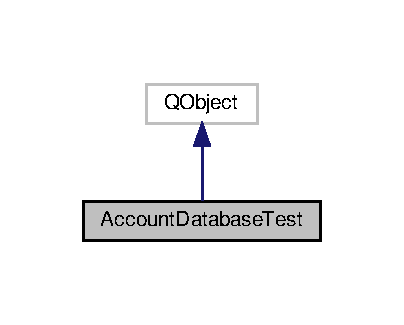
\includegraphics[width=194pt]{classAccountDatabaseTest__inherit__graph}
\end{center}
\end{figure}


Collaboration diagram for Account\+Database\+Test\+:
\nopagebreak
\begin{figure}[H]
\begin{center}
\leavevmode
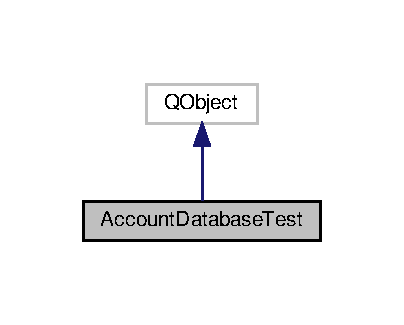
\includegraphics[width=194pt]{classAccountDatabaseTest__coll__graph}
\end{center}
\end{figure}


The documentation for this class was generated from the following file\+:\begin{DoxyCompactItemize}
\item 
test/accountdatabasetest/tst\+\_\+accountdatabasetest.\+cpp\end{DoxyCompactItemize}

\hypertarget{structAccountDatabase_1_1AccountExistsException}{}\section{Account\+Database\+:\+:Account\+Exists\+Exception Struct Reference}
\label{structAccountDatabase_1_1AccountExistsException}\index{Account\+Database\+::\+Account\+Exists\+Exception@{Account\+Database\+::\+Account\+Exists\+Exception}}


Inheritance diagram for Account\+Database\+:\+:Account\+Exists\+Exception\+:
\nopagebreak
\begin{figure}[H]
\begin{center}
\leavevmode
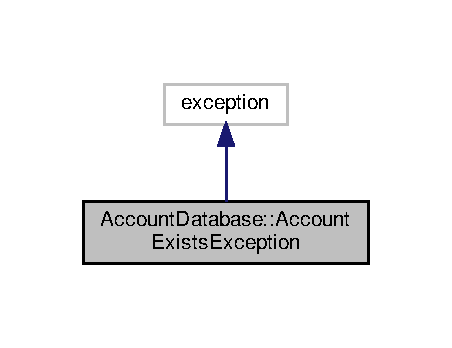
\includegraphics[width=217pt]{structAccountDatabase_1_1AccountExistsException__inherit__graph}
\end{center}
\end{figure}


Collaboration diagram for Account\+Database\+:\+:Account\+Exists\+Exception\+:
\nopagebreak
\begin{figure}[H]
\begin{center}
\leavevmode
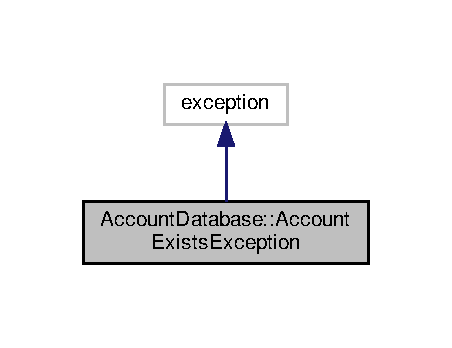
\includegraphics[width=217pt]{structAccountDatabase_1_1AccountExistsException__coll__graph}
\end{center}
\end{figure}


The documentation for this struct was generated from the following file\+:\begin{DoxyCompactItemize}
\item 
src/accountdatabase.\+h\end{DoxyCompactItemize}

\hypertarget{structAccountDatabase_1_1AccountInfo}{}\section{Account\+Database\+:\+:Account\+Info Struct Reference}
\label{structAccountDatabase_1_1AccountInfo}\index{Account\+Database\+::\+Account\+Info@{Account\+Database\+::\+Account\+Info}}


Collaboration diagram for Account\+Database\+:\+:Account\+Info\+:
\nopagebreak
\begin{figure}[H]
\begin{center}
\leavevmode
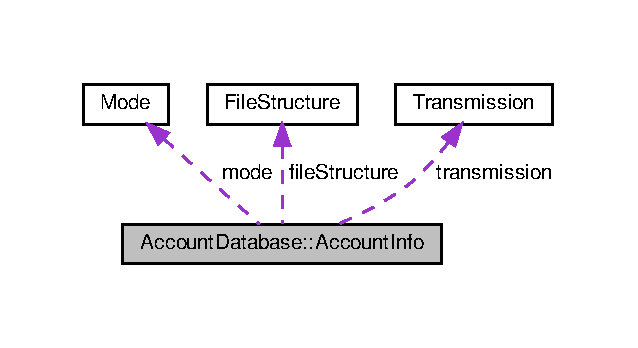
\includegraphics[width=306pt]{structAccountDatabase_1_1AccountInfo__coll__graph}
\end{center}
\end{figure}
\subsection*{Public Member Functions}
\begin{DoxyCompactItemize}
\item 
\mbox{\Hypertarget{structAccountDatabase_1_1AccountInfo_a50837455c9c85dfcd6809f7e0939f276}\label{structAccountDatabase_1_1AccountInfo_a50837455c9c85dfcd6809f7e0939f276}} 
bool {\bfseries operator==} (const \hyperlink{structAccountDatabase_1_1AccountInfo}{Account\+Info} \&a) const
\end{DoxyCompactItemize}
\subsection*{Public Attributes}
\begin{DoxyCompactItemize}
\item 
\mbox{\Hypertarget{structAccountDatabase_1_1AccountInfo_a0231e5191b13396bb9585aad8b021624}\label{structAccountDatabase_1_1AccountInfo_a0231e5191b13396bb9585aad8b021624}} 
Q\+String {\bfseries name}
\item 
\mbox{\Hypertarget{structAccountDatabase_1_1AccountInfo_a4b82b332d5ac94b77883ec2bcaa20030}\label{structAccountDatabase_1_1AccountInfo_a4b82b332d5ac94b77883ec2bcaa20030}} 
Login\+Status {\bfseries status}
\item 
\mbox{\Hypertarget{structAccountDatabase_1_1AccountInfo_af53d0d93f76edcc8092558c146297d5d}\label{structAccountDatabase_1_1AccountInfo_af53d0d93f76edcc8092558c146297d5d}} 
int {\bfseries command\+Channel\+Socket}
\item 
\mbox{\Hypertarget{structAccountDatabase_1_1AccountInfo_aac8f578c342c5692edc099e6205341c2}\label{structAccountDatabase_1_1AccountInfo_aac8f578c342c5692edc099e6205341c2}} 
int {\bfseries data\+Channel\+Socket}
\item 
\mbox{\Hypertarget{structAccountDatabase_1_1AccountInfo_a598230ee8b05e0827d767aec8abae61a}\label{structAccountDatabase_1_1AccountInfo_a598230ee8b05e0827d767aec8abae61a}} 
\hyperlink{classTransmission}{Transmission} $\ast$ {\bfseries transmission}
\item 
\mbox{\Hypertarget{structAccountDatabase_1_1AccountInfo_a0d8bf81df74545bcd28e7bc47e34e46c}\label{structAccountDatabase_1_1AccountInfo_a0d8bf81df74545bcd28e7bc47e34e46c}} 
\hyperlink{classMode}{Mode} $\ast$ {\bfseries mode}
\item 
\mbox{\Hypertarget{structAccountDatabase_1_1AccountInfo_af448b79a6f13a811408423fa9ae1c87f}\label{structAccountDatabase_1_1AccountInfo_af448b79a6f13a811408423fa9ae1c87f}} 
\hyperlink{classFileStructure}{File\+Structure} $\ast$ {\bfseries file\+Structure}
\end{DoxyCompactItemize}


The documentation for this struct was generated from the following file\+:\begin{DoxyCompactItemize}
\item 
src/accountdatabase.\+h\end{DoxyCompactItemize}

\hypertarget{structCmdUser_1_1AccountIsLoggedException}{}\section{Cmd\+User\+:\+:Account\+Is\+Logged\+Exception Struct Reference}
\label{structCmdUser_1_1AccountIsLoggedException}\index{Cmd\+User\+::\+Account\+Is\+Logged\+Exception@{Cmd\+User\+::\+Account\+Is\+Logged\+Exception}}


Inheritance diagram for Cmd\+User\+:\+:Account\+Is\+Logged\+Exception\+:
\nopagebreak
\begin{figure}[H]
\begin{center}
\leavevmode
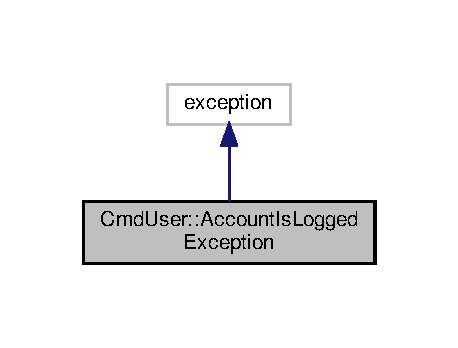
\includegraphics[width=220pt]{structCmdUser_1_1AccountIsLoggedException__inherit__graph}
\end{center}
\end{figure}


Collaboration diagram for Cmd\+User\+:\+:Account\+Is\+Logged\+Exception\+:
\nopagebreak
\begin{figure}[H]
\begin{center}
\leavevmode
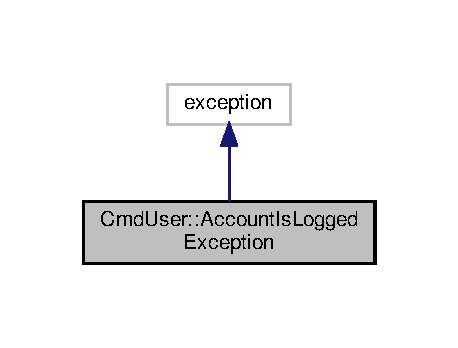
\includegraphics[width=220pt]{structCmdUser_1_1AccountIsLoggedException__coll__graph}
\end{center}
\end{figure}


The documentation for this struct was generated from the following file\+:\begin{DoxyCompactItemize}
\item 
src/cmds/cmduser.\+h\end{DoxyCompactItemize}

\hypertarget{structCmdQuit_1_1AccountIsUnloggedException}{}\section{Cmd\+Quit\+:\+:Account\+Is\+Unlogged\+Exception Struct Reference}
\label{structCmdQuit_1_1AccountIsUnloggedException}\index{Cmd\+Quit\+::\+Account\+Is\+Unlogged\+Exception@{Cmd\+Quit\+::\+Account\+Is\+Unlogged\+Exception}}


Inheritance diagram for Cmd\+Quit\+:\+:Account\+Is\+Unlogged\+Exception\+:
\nopagebreak
\begin{figure}[H]
\begin{center}
\leavevmode
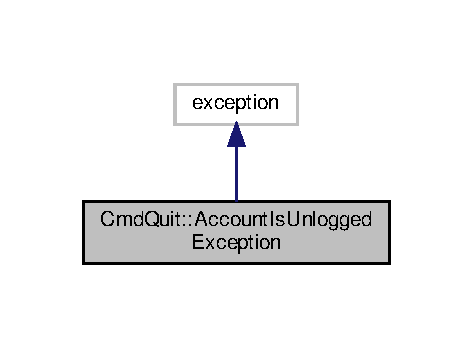
\includegraphics[width=227pt]{structCmdQuit_1_1AccountIsUnloggedException__inherit__graph}
\end{center}
\end{figure}


Collaboration diagram for Cmd\+Quit\+:\+:Account\+Is\+Unlogged\+Exception\+:
\nopagebreak
\begin{figure}[H]
\begin{center}
\leavevmode
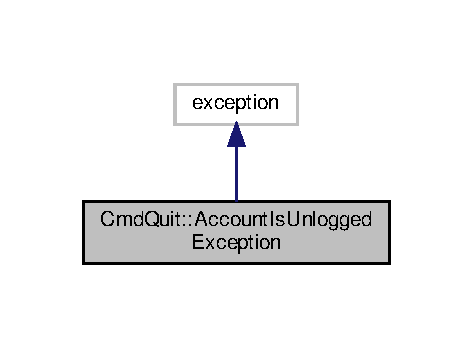
\includegraphics[width=227pt]{structCmdQuit_1_1AccountIsUnloggedException__coll__graph}
\end{center}
\end{figure}


The documentation for this struct was generated from the following file\+:\begin{DoxyCompactItemize}
\item 
src/cmds/cmdquit.\+h\end{DoxyCompactItemize}

\hypertarget{structAccountDatabase_1_1AccountNotFoundException}{}\section{Account\+Database\+:\+:Account\+Not\+Found\+Exception Struct Reference}
\label{structAccountDatabase_1_1AccountNotFoundException}\index{Account\+Database\+::\+Account\+Not\+Found\+Exception@{Account\+Database\+::\+Account\+Not\+Found\+Exception}}


Inheritance diagram for Account\+Database\+:\+:Account\+Not\+Found\+Exception\+:
\nopagebreak
\begin{figure}[H]
\begin{center}
\leavevmode
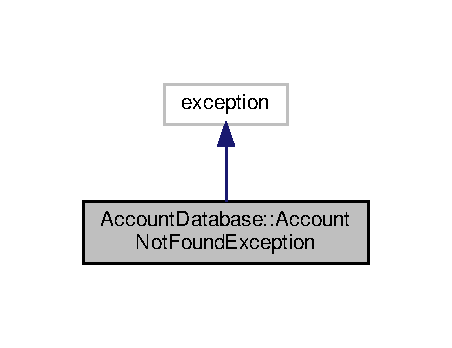
\includegraphics[width=217pt]{structAccountDatabase_1_1AccountNotFoundException__inherit__graph}
\end{center}
\end{figure}


Collaboration diagram for Account\+Database\+:\+:Account\+Not\+Found\+Exception\+:
\nopagebreak
\begin{figure}[H]
\begin{center}
\leavevmode
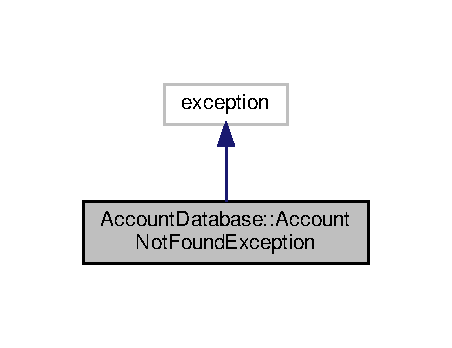
\includegraphics[width=217pt]{structAccountDatabase_1_1AccountNotFoundException__coll__graph}
\end{center}
\end{figure}


The documentation for this struct was generated from the following file\+:\begin{DoxyCompactItemize}
\item 
src/accountdatabase.\+h\end{DoxyCompactItemize}

\hypertarget{classAsciiTransmission}{}\section{Ascii\+Transmission Class Reference}
\label{classAsciiTransmission}\index{Ascii\+Transmission@{Ascii\+Transmission}}


Send or receive file through data channel in A\+S\+C\+II chars.  




{\ttfamily \#include $<$asciitransmission.\+h$>$}



Inheritance diagram for Ascii\+Transmission\+:
\nopagebreak
\begin{figure}[H]
\begin{center}
\leavevmode
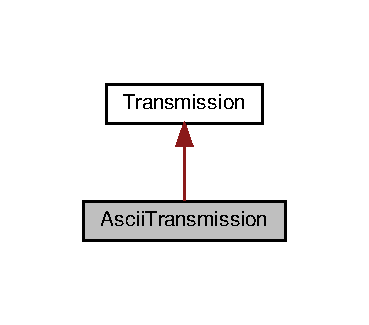
\includegraphics[width=177pt]{classAsciiTransmission__inherit__graph}
\end{center}
\end{figure}


Collaboration diagram for Ascii\+Transmission\+:
\nopagebreak
\begin{figure}[H]
\begin{center}
\leavevmode
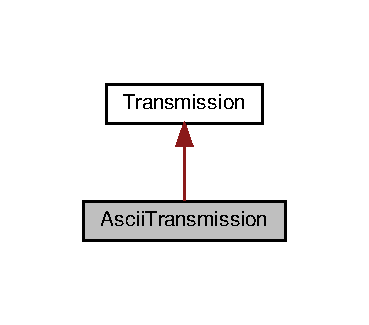
\includegraphics[width=177pt]{classAsciiTransmission__coll__graph}
\end{center}
\end{figure}
\subsection*{Public Member Functions}
\begin{DoxyCompactItemize}
\item 
\mbox{\Hypertarget{classAsciiTransmission_aa5f51d223ded66d2dfeee3120593a019}\label{classAsciiTransmission_aa5f51d223ded66d2dfeee3120593a019}} 
virtual bool {\bfseries operator==} (\hyperlink{classTransmission}{Transmission} \&transmission)=0
\end{DoxyCompactItemize}


\subsection{Detailed Description}
Send or receive file through data channel in A\+S\+C\+II chars. 

The documentation for this class was generated from the following files\+:\begin{DoxyCompactItemize}
\item 
src/transmission/types/asciitransmission.\+h\item 
src/transmission/types/asciitransmission.\+cpp\end{DoxyCompactItemize}

\hypertarget{classAsciiTransmissionReader}{}\section{Ascii\+Transmission\+Reader Class Reference}
\label{classAsciiTransmissionReader}\index{Ascii\+Transmission\+Reader@{Ascii\+Transmission\+Reader}}


Inheritance diagram for Ascii\+Transmission\+Reader\+:
\nopagebreak
\begin{figure}[H]
\begin{center}
\leavevmode
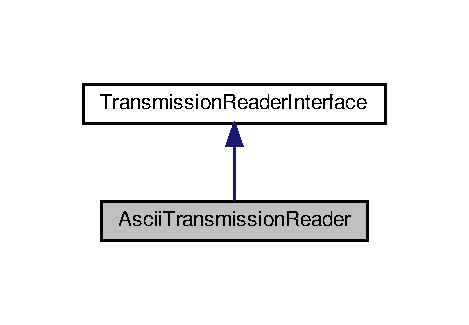
\includegraphics[width=225pt]{classAsciiTransmissionReader__inherit__graph}
\end{center}
\end{figure}


Collaboration diagram for Ascii\+Transmission\+Reader\+:
\nopagebreak
\begin{figure}[H]
\begin{center}
\leavevmode
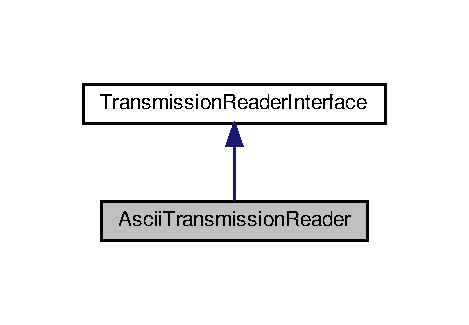
\includegraphics[width=225pt]{classAsciiTransmissionReader__coll__graph}
\end{center}
\end{figure}
\subsection*{Additional Inherited Members}


The documentation for this class was generated from the following files\+:\begin{DoxyCompactItemize}
\item 
src/transmission/types/asciitransmission.\+h\item 
src/transmission/types/asciitransmission.\+cpp\end{DoxyCompactItemize}

\hypertarget{classAsciiTransmissionWriter}{}\section{Ascii\+Transmission\+Writer Class Reference}
\label{classAsciiTransmissionWriter}\index{Ascii\+Transmission\+Writer@{Ascii\+Transmission\+Writer}}


Inheritance diagram for Ascii\+Transmission\+Writer\+:
\nopagebreak
\begin{figure}[H]
\begin{center}
\leavevmode
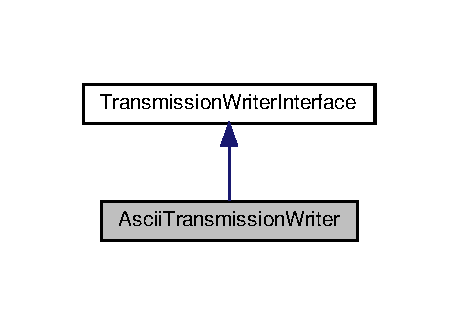
\includegraphics[width=220pt]{classAsciiTransmissionWriter__inherit__graph}
\end{center}
\end{figure}


Collaboration diagram for Ascii\+Transmission\+Writer\+:
\nopagebreak
\begin{figure}[H]
\begin{center}
\leavevmode
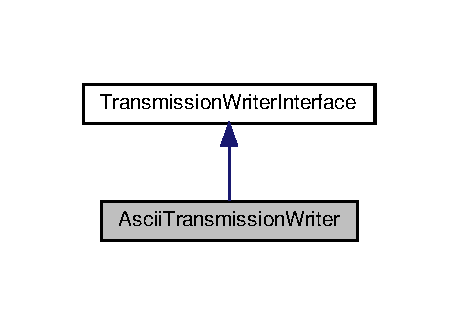
\includegraphics[width=220pt]{classAsciiTransmissionWriter__coll__graph}
\end{center}
\end{figure}
\subsection*{Additional Inherited Members}


The documentation for this class was generated from the following files\+:\begin{DoxyCompactItemize}
\item 
src/transmission/types/asciitransmission.\+h\item 
src/transmission/types/asciitransmission.\+cpp\end{DoxyCompactItemize}

\hypertarget{classBinaryTransmission}{}\section{Binary\+Transmission Class Reference}
\label{classBinaryTransmission}\index{Binary\+Transmission@{Binary\+Transmission}}


Send or receive file through data channel in binary chars.  




{\ttfamily \#include $<$binarytransmission.\+h$>$}



Inheritance diagram for Binary\+Transmission\+:
\nopagebreak
\begin{figure}[H]
\begin{center}
\leavevmode
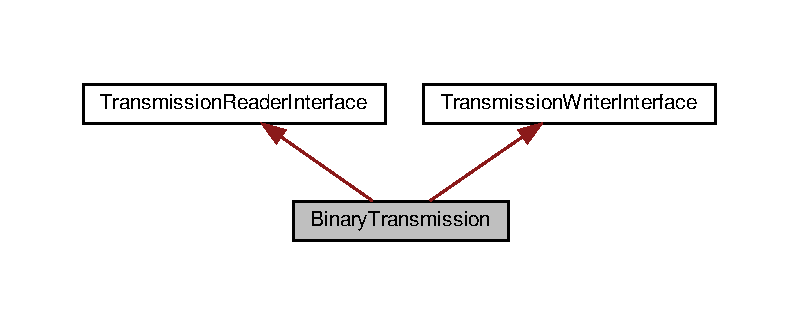
\includegraphics[width=350pt]{classBinaryTransmission__inherit__graph}
\end{center}
\end{figure}


Collaboration diagram for Binary\+Transmission\+:
\nopagebreak
\begin{figure}[H]
\begin{center}
\leavevmode
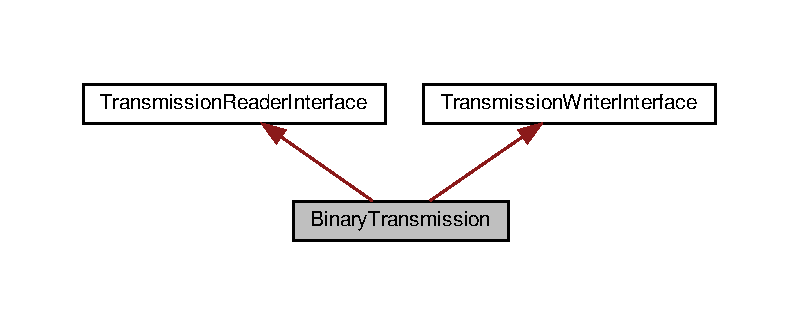
\includegraphics[width=350pt]{classBinaryTransmission__coll__graph}
\end{center}
\end{figure}
\subsection*{Public Member Functions}
\begin{DoxyCompactItemize}
\item 
\mbox{\Hypertarget{classBinaryTransmission_a48d357cdabd764fcb86022335d07c2ba}\label{classBinaryTransmission_a48d357cdabd764fcb86022335d07c2ba}} 
virtual void {\bfseries init} (const Q\+File \&file) override
\item 
\mbox{\Hypertarget{classBinaryTransmission_a319cefe379f2ae1cd069770b4aa9c765}\label{classBinaryTransmission_a319cefe379f2ae1cd069770b4aa9c765}} 
virtual Buffer \& {\bfseries read\+Data\+Portion} () override
\item 
\mbox{\Hypertarget{classBinaryTransmission_a639b12864309903735be1f4218020a7f}\label{classBinaryTransmission_a639b12864309903735be1f4218020a7f}} 
virtual bool {\bfseries is\+End\+Of\+File} () override
\item 
\mbox{\Hypertarget{classBinaryTransmission_a009c962a3e275bc0e78157e3e208e31b}\label{classBinaryTransmission_a009c962a3e275bc0e78157e3e208e31b}} 
virtual void {\bfseries clean\+Up} () override
\item 
\mbox{\Hypertarget{classBinaryTransmission_a091cecfcaca86cb7d4bd319b54723518}\label{classBinaryTransmission_a091cecfcaca86cb7d4bd319b54723518}} 
virtual bool {\bfseries operator==} (\hyperlink{classTransmission}{Transmission} \&transmission) override
\end{DoxyCompactItemize}


\subsection{Detailed Description}
Send or receive file through data channel in binary chars. 

The documentation for this class was generated from the following files\+:\begin{DoxyCompactItemize}
\item 
src/transmission/types/binarytransmission.\+h\item 
src/transmission/types/binarytransmission.\+cpp\end{DoxyCompactItemize}

\hypertarget{structCmdPort_1_1CannotConnectException}{}\section{Cmd\+Port\+:\+:Cannot\+Connect\+Exception Struct Reference}
\label{structCmdPort_1_1CannotConnectException}\index{Cmd\+Port\+::\+Cannot\+Connect\+Exception@{Cmd\+Port\+::\+Cannot\+Connect\+Exception}}


Inheritance diagram for Cmd\+Port\+:\+:Cannot\+Connect\+Exception\+:
\nopagebreak
\begin{figure}[H]
\begin{center}
\leavevmode
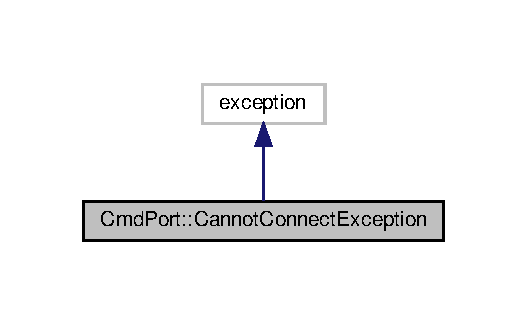
\includegraphics[width=253pt]{structCmdPort_1_1CannotConnectException__inherit__graph}
\end{center}
\end{figure}


Collaboration diagram for Cmd\+Port\+:\+:Cannot\+Connect\+Exception\+:
\nopagebreak
\begin{figure}[H]
\begin{center}
\leavevmode
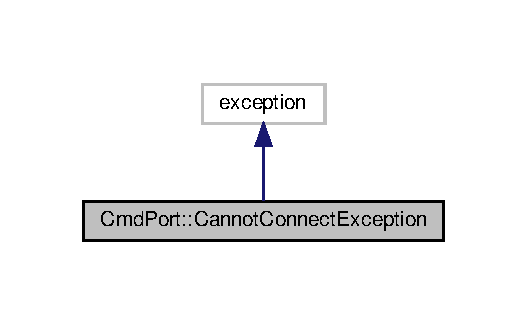
\includegraphics[width=253pt]{structCmdPort_1_1CannotConnectException__coll__graph}
\end{center}
\end{figure}


The documentation for this struct was generated from the following file\+:\begin{DoxyCompactItemize}
\item 
src/cmds/cmdport.\+h\end{DoxyCompactItemize}

\hypertarget{classCmdMode}{}\section{Cmd\+Mode Class Reference}
\label{classCmdMode}\index{Cmd\+Mode@{Cmd\+Mode}}


Inheritance diagram for Cmd\+Mode\+:
\nopagebreak
\begin{figure}[H]
\begin{center}
\leavevmode
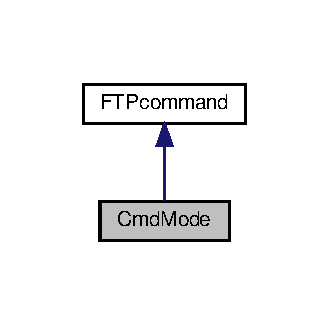
\includegraphics[width=158pt]{classCmdMode__inherit__graph}
\end{center}
\end{figure}


Collaboration diagram for Cmd\+Mode\+:
\nopagebreak
\begin{figure}[H]
\begin{center}
\leavevmode
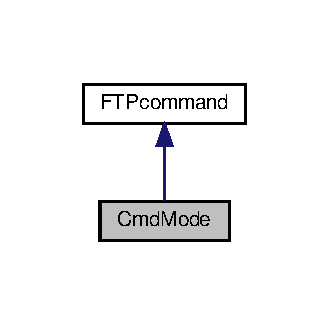
\includegraphics[width=158pt]{classCmdMode__coll__graph}
\end{center}
\end{figure}
\subsection*{Public Types}
\begin{DoxyCompactItemize}
\item 
\mbox{\Hypertarget{classCmdMode_ad8aa7ec04fa921d1036cd2568dbe15a0}\label{classCmdMode_ad8aa7ec04fa921d1036cd2568dbe15a0}} 
using {\bfseries Account\+Not\+Found\+Exception} = \hyperlink{structAccountDatabase_1_1AccountNotFoundException}{Account\+Database\+::\+Account\+Not\+Found\+Exception}
\end{DoxyCompactItemize}
\subsection*{Public Member Functions}
\begin{DoxyCompactItemize}
\item 
\hyperlink{classCmdMode_a3786de8e982eb68113e80ee6966eb9cf}{Cmd\+Mode} (int command\+Channel\+Socket, \hyperlink{classMode}{Mode} $\ast$const mode)
\begin{DoxyCompactList}\small\item\em \hyperlink{classCmdPort}{Cmd\+Port}. \end{DoxyCompactList}\item 
\mbox{\Hypertarget{classCmdMode_ad00abfad98d5aa888f13e55366f6dc5e}\label{classCmdMode_ad00abfad98d5aa888f13e55366f6dc5e}} 
void {\bfseries execute} () override
\end{DoxyCompactItemize}
\subsection*{Additional Inherited Members}


\subsection{Constructor \& Destructor Documentation}
\mbox{\Hypertarget{classCmdMode_a3786de8e982eb68113e80ee6966eb9cf}\label{classCmdMode_a3786de8e982eb68113e80ee6966eb9cf}} 
\index{Cmd\+Mode@{Cmd\+Mode}!Cmd\+Mode@{Cmd\+Mode}}
\index{Cmd\+Mode@{Cmd\+Mode}!Cmd\+Mode@{Cmd\+Mode}}
\subsubsection{\texorpdfstring{Cmd\+Mode()}{CmdMode()}}
{\footnotesize\ttfamily Cmd\+Mode\+::\+Cmd\+Mode (\begin{DoxyParamCaption}\item[{int}]{command\+Channel\+Socket,  }\item[{\hyperlink{classMode}{Mode} $\ast$const}]{mode }\end{DoxyParamCaption})}



\hyperlink{classCmdPort}{Cmd\+Port}. 


\begin{DoxyParams}{Parameters}
{\em command\+Channel\+Socket} & Client command channel socket \\
\hline
{\em mode} & Type of mode \\
\hline
\end{DoxyParams}


The documentation for this class was generated from the following files\+:\begin{DoxyCompactItemize}
\item 
src/cmds/cmdmode.\+h\item 
src/cmds/cmdmode.\+cpp\end{DoxyCompactItemize}

\hypertarget{classCmdModeTest}{}\section{Cmd\+Mode\+Test Class Reference}
\label{classCmdModeTest}\index{Cmd\+Mode\+Test@{Cmd\+Mode\+Test}}


Inheritance diagram for Cmd\+Mode\+Test\+:
\nopagebreak
\begin{figure}[H]
\begin{center}
\leavevmode
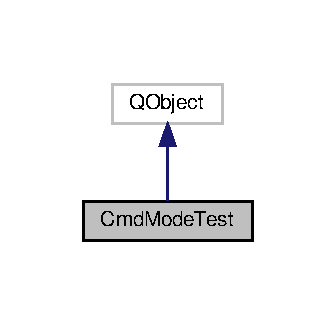
\includegraphics[width=161pt]{classCmdModeTest__inherit__graph}
\end{center}
\end{figure}


Collaboration diagram for Cmd\+Mode\+Test\+:
\nopagebreak
\begin{figure}[H]
\begin{center}
\leavevmode
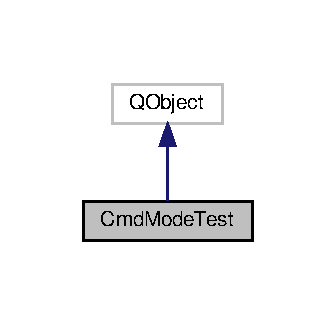
\includegraphics[width=161pt]{classCmdModeTest__coll__graph}
\end{center}
\end{figure}


The documentation for this class was generated from the following file\+:\begin{DoxyCompactItemize}
\item 
test/cmdmodetest/tst\+\_\+cmdmodetest.\+cpp\end{DoxyCompactItemize}

\hypertarget{classCmdPort}{}\section{Cmd\+Port Class Reference}
\label{classCmdPort}\index{Cmd\+Port@{Cmd\+Port}}


Inheritance diagram for Cmd\+Port\+:
\nopagebreak
\begin{figure}[H]
\begin{center}
\leavevmode
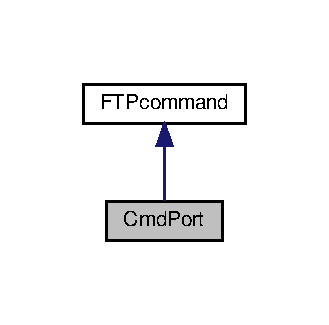
\includegraphics[width=158pt]{classCmdPort__inherit__graph}
\end{center}
\end{figure}


Collaboration diagram for Cmd\+Port\+:
\nopagebreak
\begin{figure}[H]
\begin{center}
\leavevmode
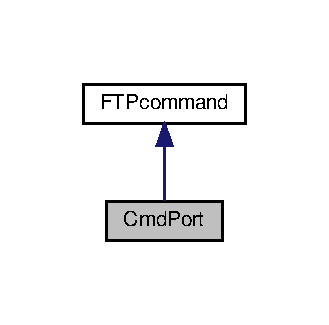
\includegraphics[width=158pt]{classCmdPort__coll__graph}
\end{center}
\end{figure}
\subsection*{Classes}
\begin{DoxyCompactItemize}
\item 
struct \hyperlink{structCmdPort_1_1CannotConnectException}{Cannot\+Connect\+Exception}
\item 
struct \hyperlink{structCmdPort_1_1DataChannelSocketNotExistsException}{Data\+Channel\+Socket\+Not\+Exists\+Exception}
\end{DoxyCompactItemize}
\subsection*{Public Types}
\begin{DoxyCompactItemize}
\item 
\mbox{\Hypertarget{classCmdPort_a52b57e3d2984f4198fdbcb235e46509e}\label{classCmdPort_a52b57e3d2984f4198fdbcb235e46509e}} 
using {\bfseries Account\+Not\+Found\+Exception} = \hyperlink{structAccountDatabase_1_1AccountNotFoundException}{Account\+Database\+::\+Account\+Not\+Found\+Exception}
\end{DoxyCompactItemize}
\subsection*{Public Member Functions}
\begin{DoxyCompactItemize}
\item 
\hyperlink{classCmdPort_a81f0136aa4cd9364e5998fffd703876f}{Cmd\+Port} (int command\+Channel\+Socket, sockaddr\+\_\+in address)
\begin{DoxyCompactList}\small\item\em \hyperlink{classCmdPort}{Cmd\+Port}. \end{DoxyCompactList}\item 
\mbox{\Hypertarget{classCmdPort_a3b43d863b32447013c0e8ae5b7035914}\label{classCmdPort_a3b43d863b32447013c0e8ae5b7035914}} 
void {\bfseries execute} () override
\item 
\mbox{\Hypertarget{classCmdPort_abbe13bd8440f5cbf0c16aa0bff57d4ad}\label{classCmdPort_abbe13bd8440f5cbf0c16aa0bff57d4ad}} 
int {\bfseries get\+Data\+Channel\+Socket} () const
\end{DoxyCompactItemize}
\subsection*{Additional Inherited Members}


\subsection{Constructor \& Destructor Documentation}
\mbox{\Hypertarget{classCmdPort_a81f0136aa4cd9364e5998fffd703876f}\label{classCmdPort_a81f0136aa4cd9364e5998fffd703876f}} 
\index{Cmd\+Port@{Cmd\+Port}!Cmd\+Port@{Cmd\+Port}}
\index{Cmd\+Port@{Cmd\+Port}!Cmd\+Port@{Cmd\+Port}}
\subsubsection{\texorpdfstring{Cmd\+Port()}{CmdPort()}}
{\footnotesize\ttfamily Cmd\+Port\+::\+Cmd\+Port (\begin{DoxyParamCaption}\item[{int}]{command\+Channel\+Socket,  }\item[{sockaddr\+\_\+in}]{address }\end{DoxyParamCaption})}



\hyperlink{classCmdPort}{Cmd\+Port}. 


\begin{DoxyParams}{Parameters}
{\em command\+Channel\+Socket} & Client command channel socket \\
\hline
{\em address} & Client data communication channel address \\
\hline
\end{DoxyParams}


The documentation for this class was generated from the following files\+:\begin{DoxyCompactItemize}
\item 
src/cmds/cmdport.\+h\item 
src/cmds/cmdport.\+cpp\end{DoxyCompactItemize}

\hypertarget{classCmdPortTest}{}\section{Cmd\+Port\+Test Class Reference}
\label{classCmdPortTest}\index{Cmd\+Port\+Test@{Cmd\+Port\+Test}}


Inheritance diagram for Cmd\+Port\+Test\+:
\nopagebreak
\begin{figure}[H]
\begin{center}
\leavevmode
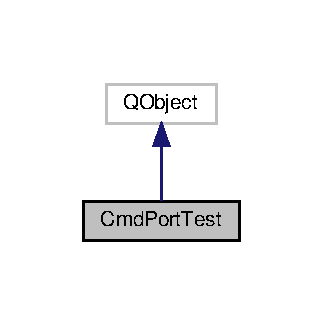
\includegraphics[width=155pt]{classCmdPortTest__inherit__graph}
\end{center}
\end{figure}


Collaboration diagram for Cmd\+Port\+Test\+:
\nopagebreak
\begin{figure}[H]
\begin{center}
\leavevmode
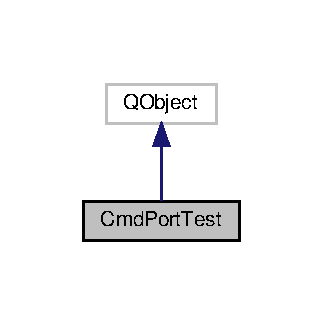
\includegraphics[width=155pt]{classCmdPortTest__coll__graph}
\end{center}
\end{figure}


The documentation for this class was generated from the following file\+:\begin{DoxyCompactItemize}
\item 
test/cmdporttest/tst\+\_\+cmdporttest.\+cpp\end{DoxyCompactItemize}

\hypertarget{classCmdQuit}{}\section{Cmd\+Quit Class Reference}
\label{classCmdQuit}\index{Cmd\+Quit@{Cmd\+Quit}}


Sign out a logged client.  




{\ttfamily \#include $<$cmdquit.\+h$>$}



Inheritance diagram for Cmd\+Quit\+:
\nopagebreak
\begin{figure}[H]
\begin{center}
\leavevmode
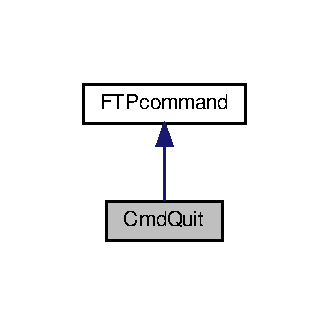
\includegraphics[width=158pt]{classCmdQuit__inherit__graph}
\end{center}
\end{figure}


Collaboration diagram for Cmd\+Quit\+:
\nopagebreak
\begin{figure}[H]
\begin{center}
\leavevmode
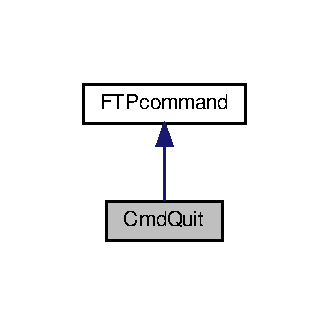
\includegraphics[width=158pt]{classCmdQuit__coll__graph}
\end{center}
\end{figure}
\subsection*{Classes}
\begin{DoxyCompactItemize}
\item 
struct \hyperlink{structCmdQuit_1_1AccountIsUnloggedException}{Account\+Is\+Unlogged\+Exception}
\end{DoxyCompactItemize}
\subsection*{Public Types}
\begin{DoxyCompactItemize}
\item 
\mbox{\Hypertarget{classCmdQuit_ae65ce68209e37afaa75e5a97c6202a1a}\label{classCmdQuit_ae65ce68209e37afaa75e5a97c6202a1a}} 
using {\bfseries Account\+Not\+Found\+Exception} = \hyperlink{structAccountDatabase_1_1AccountNotFoundException}{Account\+Database\+::\+Account\+Not\+Found\+Exception}
\end{DoxyCompactItemize}
\subsection*{Public Member Functions}
\begin{DoxyCompactItemize}
\item 
\hyperlink{classCmdQuit_abab586b6df59ad1fcb59150ca2b72d97}{Cmd\+Quit} (int command\+Channel\+Socket)
\begin{DoxyCompactList}\small\item\em \hyperlink{classCmdQuit}{Cmd\+Quit}. \end{DoxyCompactList}\item 
\mbox{\Hypertarget{classCmdQuit_acf50df91ad695a40a449890300344f4b}\label{classCmdQuit_acf50df91ad695a40a449890300344f4b}} 
void {\bfseries execute} () override
\end{DoxyCompactItemize}
\subsection*{Additional Inherited Members}


\subsection{Detailed Description}
Sign out a logged client. 

\subsection{Constructor \& Destructor Documentation}
\mbox{\Hypertarget{classCmdQuit_abab586b6df59ad1fcb59150ca2b72d97}\label{classCmdQuit_abab586b6df59ad1fcb59150ca2b72d97}} 
\index{Cmd\+Quit@{Cmd\+Quit}!Cmd\+Quit@{Cmd\+Quit}}
\index{Cmd\+Quit@{Cmd\+Quit}!Cmd\+Quit@{Cmd\+Quit}}
\subsubsection{\texorpdfstring{Cmd\+Quit()}{CmdQuit()}}
{\footnotesize\ttfamily Cmd\+Quit\+::\+Cmd\+Quit (\begin{DoxyParamCaption}\item[{int}]{command\+Channel\+Socket }\end{DoxyParamCaption})}



\hyperlink{classCmdQuit}{Cmd\+Quit}. 


\begin{DoxyParams}{Parameters}
{\em command\+Channel\+Socket} & Socket to communication with client on command channel \\
\hline
\end{DoxyParams}


The documentation for this class was generated from the following files\+:\begin{DoxyCompactItemize}
\item 
src/cmds/cmdquit.\+h\item 
src/cmds/cmdquit.\+cpp\end{DoxyCompactItemize}

\hypertarget{classCmdQuitTest}{}\section{Cmd\+Quit\+Test Class Reference}
\label{classCmdQuitTest}\index{Cmd\+Quit\+Test@{Cmd\+Quit\+Test}}


Inheritance diagram for Cmd\+Quit\+Test\+:
\nopagebreak
\begin{figure}[H]
\begin{center}
\leavevmode
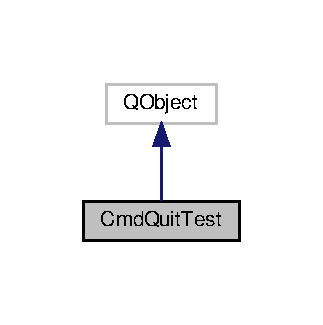
\includegraphics[width=155pt]{classCmdQuitTest__inherit__graph}
\end{center}
\end{figure}


Collaboration diagram for Cmd\+Quit\+Test\+:
\nopagebreak
\begin{figure}[H]
\begin{center}
\leavevmode
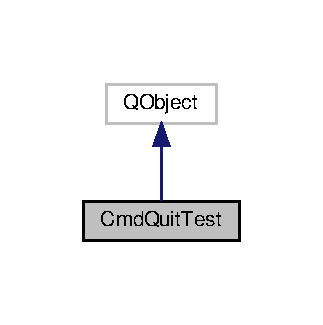
\includegraphics[width=155pt]{classCmdQuitTest__coll__graph}
\end{center}
\end{figure}


The documentation for this class was generated from the following file\+:\begin{DoxyCompactItemize}
\item 
test/cmdquittest/tst\+\_\+cmdquittest.\+cpp\end{DoxyCompactItemize}

\hypertarget{classCmdStru}{}\section{Cmd\+Stru Class Reference}
\label{classCmdStru}\index{Cmd\+Stru@{Cmd\+Stru}}


Inheritance diagram for Cmd\+Stru\+:
\nopagebreak
\begin{figure}[H]
\begin{center}
\leavevmode
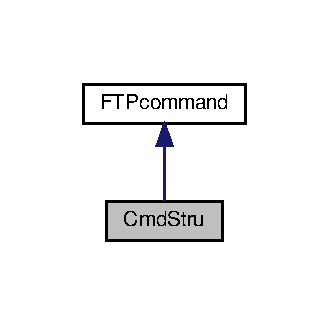
\includegraphics[width=158pt]{classCmdStru__inherit__graph}
\end{center}
\end{figure}


Collaboration diagram for Cmd\+Stru\+:
\nopagebreak
\begin{figure}[H]
\begin{center}
\leavevmode
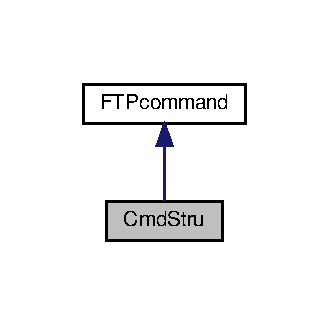
\includegraphics[width=158pt]{classCmdStru__coll__graph}
\end{center}
\end{figure}
\subsection*{Public Types}
\begin{DoxyCompactItemize}
\item 
\mbox{\Hypertarget{classCmdStru_a5ad00a8aeb7ee1e9468026e55120ada2}\label{classCmdStru_a5ad00a8aeb7ee1e9468026e55120ada2}} 
using {\bfseries Account\+Not\+Found\+Exception} = \hyperlink{structAccountDatabase_1_1AccountNotFoundException}{Account\+Database\+::\+Account\+Not\+Found\+Exception}
\end{DoxyCompactItemize}
\subsection*{Public Member Functions}
\begin{DoxyCompactItemize}
\item 
\hyperlink{classCmdStru_a1c3d22047704a9f0fc24015287f3a356}{Cmd\+Stru} (int command\+Channel\+Socket, \hyperlink{classFileStructure}{File\+Structure} $\ast$const file\+Structure)
\begin{DoxyCompactList}\small\item\em \hyperlink{classCmdQuit}{Cmd\+Quit}. \end{DoxyCompactList}\item 
\mbox{\Hypertarget{classCmdStru_acda350a5abfd38670ad0fb337d651e4d}\label{classCmdStru_acda350a5abfd38670ad0fb337d651e4d}} 
void {\bfseries execute} () override
\end{DoxyCompactItemize}
\subsection*{Additional Inherited Members}


\subsection{Constructor \& Destructor Documentation}
\mbox{\Hypertarget{classCmdStru_a1c3d22047704a9f0fc24015287f3a356}\label{classCmdStru_a1c3d22047704a9f0fc24015287f3a356}} 
\index{Cmd\+Stru@{Cmd\+Stru}!Cmd\+Stru@{Cmd\+Stru}}
\index{Cmd\+Stru@{Cmd\+Stru}!Cmd\+Stru@{Cmd\+Stru}}
\subsubsection{\texorpdfstring{Cmd\+Stru()}{CmdStru()}}
{\footnotesize\ttfamily Cmd\+Stru\+::\+Cmd\+Stru (\begin{DoxyParamCaption}\item[{int}]{command\+Channel\+Socket,  }\item[{\hyperlink{classFileStructure}{File\+Structure} $\ast$const}]{file\+Structure }\end{DoxyParamCaption})}



\hyperlink{classCmdQuit}{Cmd\+Quit}. 


\begin{DoxyParams}{Parameters}
{\em command\+Channel\+Socket} & Socket to communication with client on command channel \\
\hline
{\em file\+Structure} & Type of files structure \\
\hline
\end{DoxyParams}


The documentation for this class was generated from the following files\+:\begin{DoxyCompactItemize}
\item 
src/cmds/cmdstru.\+h\item 
src/cmds/cmdstru.\+cpp\end{DoxyCompactItemize}

\hypertarget{classCmdStruTest}{}\section{Cmd\+Stru\+Test Class Reference}
\label{classCmdStruTest}\index{Cmd\+Stru\+Test@{Cmd\+Stru\+Test}}


Inheritance diagram for Cmd\+Stru\+Test\+:
\nopagebreak
\begin{figure}[H]
\begin{center}
\leavevmode
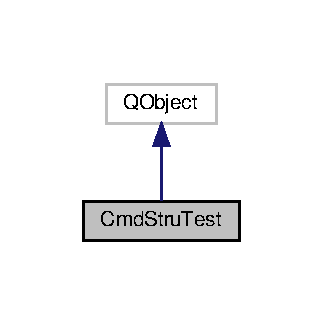
\includegraphics[width=155pt]{classCmdStruTest__inherit__graph}
\end{center}
\end{figure}


Collaboration diagram for Cmd\+Stru\+Test\+:
\nopagebreak
\begin{figure}[H]
\begin{center}
\leavevmode
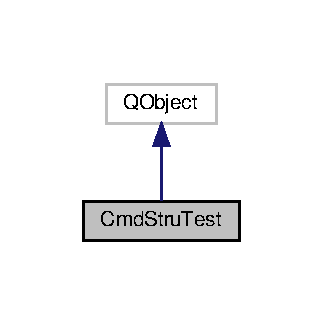
\includegraphics[width=155pt]{classCmdStruTest__coll__graph}
\end{center}
\end{figure}


The documentation for this class was generated from the following file\+:\begin{DoxyCompactItemize}
\item 
test/cmdstru/tst\+\_\+cmdstrutest.\+cpp\end{DoxyCompactItemize}

\hypertarget{classCmdType}{}\section{Cmd\+Type Class Reference}
\label{classCmdType}\index{Cmd\+Type@{Cmd\+Type}}


Change type of transmission.  




{\ttfamily \#include $<$cmdtype.\+h$>$}



Inheritance diagram for Cmd\+Type\+:
\nopagebreak
\begin{figure}[H]
\begin{center}
\leavevmode
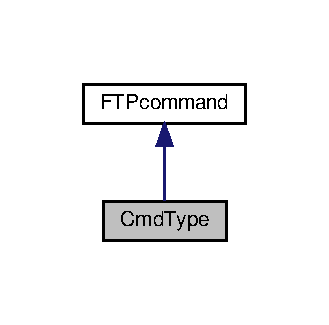
\includegraphics[width=158pt]{classCmdType__inherit__graph}
\end{center}
\end{figure}


Collaboration diagram for Cmd\+Type\+:
\nopagebreak
\begin{figure}[H]
\begin{center}
\leavevmode
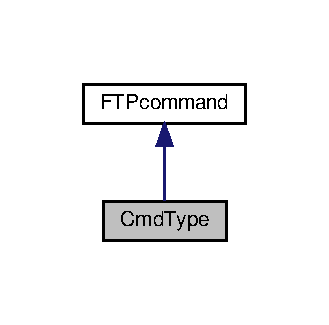
\includegraphics[width=158pt]{classCmdType__coll__graph}
\end{center}
\end{figure}
\subsection*{Public Types}
\begin{DoxyCompactItemize}
\item 
\mbox{\Hypertarget{classCmdType_a3183eef703d97624611bf756a58ee5fa}\label{classCmdType_a3183eef703d97624611bf756a58ee5fa}} 
using {\bfseries Account\+Not\+Found\+Exception} = \hyperlink{structAccountDatabase_1_1AccountNotFoundException}{Account\+Database\+::\+Account\+Not\+Found\+Exception}
\end{DoxyCompactItemize}
\subsection*{Public Member Functions}
\begin{DoxyCompactItemize}
\item 
\hyperlink{classCmdType_a5e667300d7e4ae811601ce120708423f}{Cmd\+Type} (int command\+Channel\+Socket, \hyperlink{classTransmission}{Transmission} $\ast$const transmission)
\begin{DoxyCompactList}\small\item\em \hyperlink{classCmdQuit}{Cmd\+Quit}. \end{DoxyCompactList}\item 
\mbox{\Hypertarget{classCmdType_a5d8e3af14974a4fc05356d8af008463d}\label{classCmdType_a5d8e3af14974a4fc05356d8af008463d}} 
void {\bfseries execute} () override
\end{DoxyCompactItemize}
\subsection*{Additional Inherited Members}


\subsection{Detailed Description}
Change type of transmission. 

\subsection{Constructor \& Destructor Documentation}
\mbox{\Hypertarget{classCmdType_a5e667300d7e4ae811601ce120708423f}\label{classCmdType_a5e667300d7e4ae811601ce120708423f}} 
\index{Cmd\+Type@{Cmd\+Type}!Cmd\+Type@{Cmd\+Type}}
\index{Cmd\+Type@{Cmd\+Type}!Cmd\+Type@{Cmd\+Type}}
\subsubsection{\texorpdfstring{Cmd\+Type()}{CmdType()}}
{\footnotesize\ttfamily Cmd\+Type\+::\+Cmd\+Type (\begin{DoxyParamCaption}\item[{int}]{command\+Channel\+Socket,  }\item[{\hyperlink{classTransmission}{Transmission} $\ast$const}]{transmission }\end{DoxyParamCaption})}



\hyperlink{classCmdQuit}{Cmd\+Quit}. 


\begin{DoxyParams}{Parameters}
{\em command\+Channel\+Socket} & Socket to communication with client on command channel \\
\hline
{\em transmission} & Type of transmission \\
\hline
\end{DoxyParams}


The documentation for this class was generated from the following files\+:\begin{DoxyCompactItemize}
\item 
src/cmds/cmdtype.\+h\item 
src/cmds/cmdtype.\+cpp\end{DoxyCompactItemize}

\hypertarget{classCmdTypeTest}{}\section{Cmd\+Type\+Test Class Reference}
\label{classCmdTypeTest}\index{Cmd\+Type\+Test@{Cmd\+Type\+Test}}


Inheritance diagram for Cmd\+Type\+Test\+:
\nopagebreak
\begin{figure}[H]
\begin{center}
\leavevmode
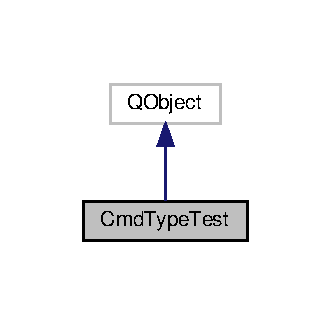
\includegraphics[width=159pt]{classCmdTypeTest__inherit__graph}
\end{center}
\end{figure}


Collaboration diagram for Cmd\+Type\+Test\+:
\nopagebreak
\begin{figure}[H]
\begin{center}
\leavevmode
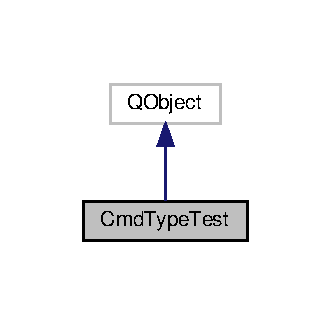
\includegraphics[width=159pt]{classCmdTypeTest__coll__graph}
\end{center}
\end{figure}


The documentation for this class was generated from the following file\+:\begin{DoxyCompactItemize}
\item 
test/cmdtypetest/tst\+\_\+cmdtypetest.\+cpp\end{DoxyCompactItemize}

\hypertarget{classCmdUser}{}\section{Cmd\+User Class Reference}
\label{classCmdUser}\index{Cmd\+User@{Cmd\+User}}


Creates a new account or sign in a client.  




{\ttfamily \#include $<$cmduser.\+h$>$}



Inheritance diagram for Cmd\+User\+:
\nopagebreak
\begin{figure}[H]
\begin{center}
\leavevmode
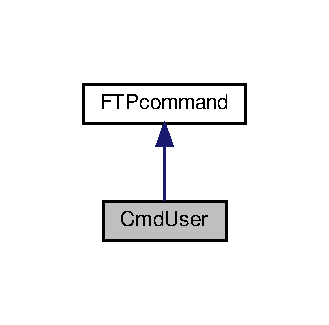
\includegraphics[width=158pt]{classCmdUser__inherit__graph}
\end{center}
\end{figure}


Collaboration diagram for Cmd\+User\+:
\nopagebreak
\begin{figure}[H]
\begin{center}
\leavevmode
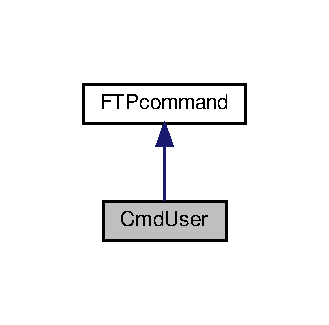
\includegraphics[width=158pt]{classCmdUser__coll__graph}
\end{center}
\end{figure}
\subsection*{Classes}
\begin{DoxyCompactItemize}
\item 
struct \hyperlink{structCmdUser_1_1AccountIsLoggedException}{Account\+Is\+Logged\+Exception}
\end{DoxyCompactItemize}
\subsection*{Public Member Functions}
\begin{DoxyCompactItemize}
\item 
\hyperlink{classCmdUser_a97e1717dbed581a67d86de3102ba6933}{Cmd\+User} (Q\+String name, int command\+Channel\+Socket)
\begin{DoxyCompactList}\small\item\em \hyperlink{classCmdUser}{Cmd\+User}. \end{DoxyCompactList}\item 
\mbox{\Hypertarget{classCmdUser_af23e5db7b5f2b3dcef89e26dba8f980c}\label{classCmdUser_af23e5db7b5f2b3dcef89e26dba8f980c}} 
void {\bfseries execute} () override
\end{DoxyCompactItemize}
\subsection*{Additional Inherited Members}


\subsection{Detailed Description}
Creates a new account or sign in a client. 

\subsection{Constructor \& Destructor Documentation}
\mbox{\Hypertarget{classCmdUser_a97e1717dbed581a67d86de3102ba6933}\label{classCmdUser_a97e1717dbed581a67d86de3102ba6933}} 
\index{Cmd\+User@{Cmd\+User}!Cmd\+User@{Cmd\+User}}
\index{Cmd\+User@{Cmd\+User}!Cmd\+User@{Cmd\+User}}
\subsubsection{\texorpdfstring{Cmd\+User()}{CmdUser()}}
{\footnotesize\ttfamily Cmd\+User\+::\+Cmd\+User (\begin{DoxyParamCaption}\item[{Q\+String}]{name,  }\item[{int}]{command\+Channel\+Socket }\end{DoxyParamCaption})}



\hyperlink{classCmdUser}{Cmd\+User}. 


\begin{DoxyParams}{Parameters}
{\em name} & Client name \\
\hline
{\em command\+Channel\+Socket} & Socket to communication with client on command channel \\
\hline
\end{DoxyParams}


The documentation for this class was generated from the following files\+:\begin{DoxyCompactItemize}
\item 
src/cmds/cmduser.\+h\item 
src/cmds/cmduser.\+cpp\end{DoxyCompactItemize}

\hypertarget{classCmdUserTest}{}\section{Cmd\+User\+Test Class Reference}
\label{classCmdUserTest}\index{Cmd\+User\+Test@{Cmd\+User\+Test}}


Inheritance diagram for Cmd\+User\+Test\+:
\nopagebreak
\begin{figure}[H]
\begin{center}
\leavevmode
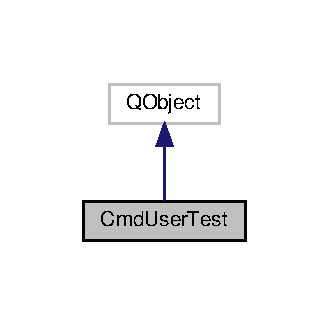
\includegraphics[width=158pt]{classCmdUserTest__inherit__graph}
\end{center}
\end{figure}


Collaboration diagram for Cmd\+User\+Test\+:
\nopagebreak
\begin{figure}[H]
\begin{center}
\leavevmode
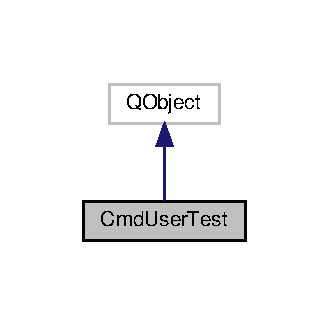
\includegraphics[width=158pt]{classCmdUserTest__coll__graph}
\end{center}
\end{figure}


The documentation for this class was generated from the following file\+:\begin{DoxyCompactItemize}
\item 
test/cmdusertest/tst\+\_\+cmdusertest.\+cpp\end{DoxyCompactItemize}

\hypertarget{structCmdPort_1_1DataChannelSocketNotExistsException}{}\section{Cmd\+Port\+:\+:Data\+Channel\+Socket\+Not\+Exists\+Exception Struct Reference}
\label{structCmdPort_1_1DataChannelSocketNotExistsException}\index{Cmd\+Port\+::\+Data\+Channel\+Socket\+Not\+Exists\+Exception@{Cmd\+Port\+::\+Data\+Channel\+Socket\+Not\+Exists\+Exception}}


Inheritance diagram for Cmd\+Port\+:\+:Data\+Channel\+Socket\+Not\+Exists\+Exception\+:
\nopagebreak
\begin{figure}[H]
\begin{center}
\leavevmode
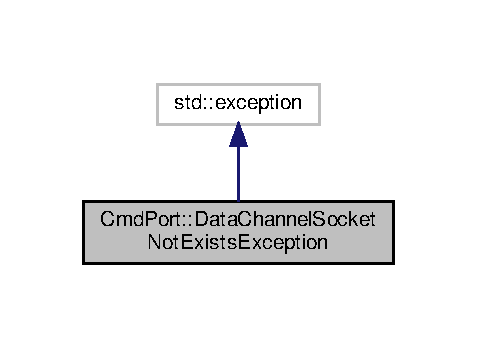
\includegraphics[width=229pt]{structCmdPort_1_1DataChannelSocketNotExistsException__inherit__graph}
\end{center}
\end{figure}


Collaboration diagram for Cmd\+Port\+:\+:Data\+Channel\+Socket\+Not\+Exists\+Exception\+:
\nopagebreak
\begin{figure}[H]
\begin{center}
\leavevmode
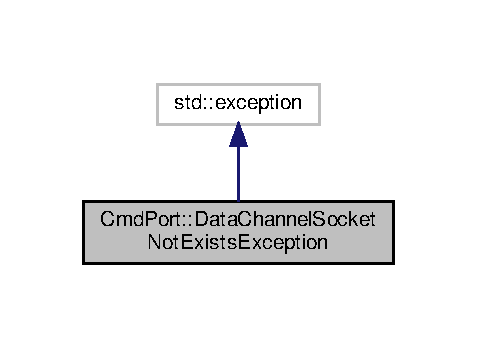
\includegraphics[width=229pt]{structCmdPort_1_1DataChannelSocketNotExistsException__coll__graph}
\end{center}
\end{figure}


The documentation for this struct was generated from the following file\+:\begin{DoxyCompactItemize}
\item 
src/cmds/cmdport.\+h\end{DoxyCompactItemize}

\hypertarget{classFakeClassA}{}\section{Fake\+ClassA Class Reference}
\label{classFakeClassA}\index{Fake\+ClassA@{Fake\+ClassA}}


Inheritance diagram for Fake\+ClassA\+:
\nopagebreak
\begin{figure}[H]
\begin{center}
\leavevmode
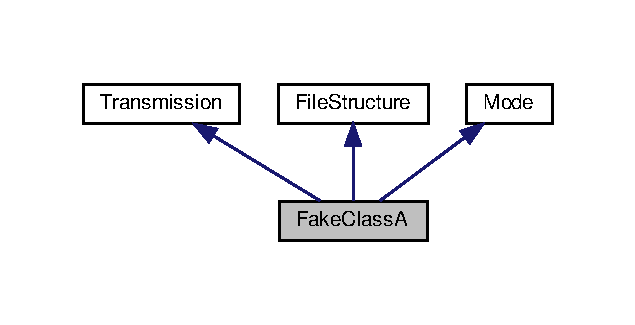
\includegraphics[width=305pt]{classFakeClassA__inherit__graph}
\end{center}
\end{figure}


Collaboration diagram for Fake\+ClassA\+:
\nopagebreak
\begin{figure}[H]
\begin{center}
\leavevmode
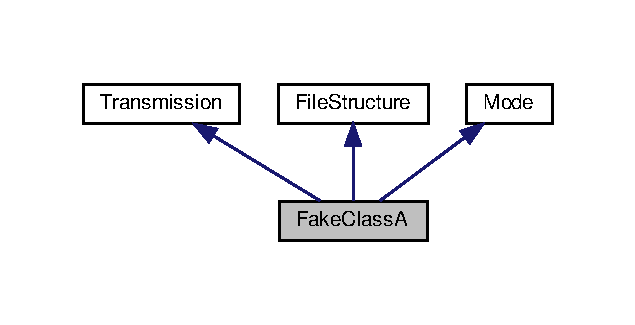
\includegraphics[width=305pt]{classFakeClassA__coll__graph}
\end{center}
\end{figure}
\subsection*{Additional Inherited Members}


The documentation for this class was generated from the following files\+:\begin{DoxyCompactItemize}
\item 
test/cmdmodetest/Fake\+Mode\+Classes.\+h\item 
test/cmdstru/Fake\+File\+Structure\+Classes.\+h\item 
test/cmdtypetest/Fake\+Transmission\+Classes.\+h\end{DoxyCompactItemize}

\hypertarget{classFakeClassB}{}\section{Fake\+ClassB Class Reference}
\label{classFakeClassB}\index{Fake\+ClassB@{Fake\+ClassB}}


Inheritance diagram for Fake\+ClassB\+:
\nopagebreak
\begin{figure}[H]
\begin{center}
\leavevmode
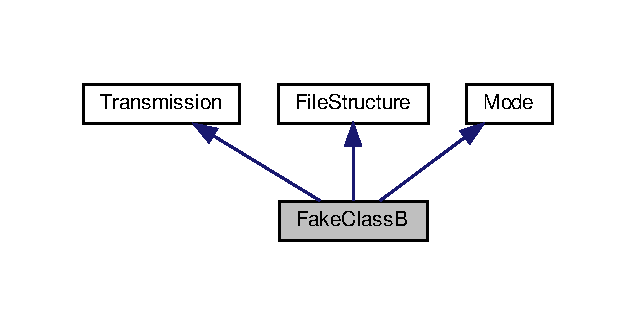
\includegraphics[width=305pt]{classFakeClassB__inherit__graph}
\end{center}
\end{figure}


Collaboration diagram for Fake\+ClassB\+:
\nopagebreak
\begin{figure}[H]
\begin{center}
\leavevmode
\includegraphics[width=305pt]{classFakeClassB__coll__graph}
\end{center}
\end{figure}
\subsection*{Additional Inherited Members}


The documentation for this class was generated from the following files\+:\begin{DoxyCompactItemize}
\item 
test/cmdmodetest/Fake\+Mode\+Classes.\+h\item 
test/cmdstru/Fake\+File\+Structure\+Classes.\+h\item 
test/cmdtypetest/Fake\+Transmission\+Classes.\+h\end{DoxyCompactItemize}

\hypertarget{classFakeClientDataServer}{}\section{Fake\+Client\+Data\+Server Class Reference}
\label{classFakeClientDataServer}\index{Fake\+Client\+Data\+Server@{Fake\+Client\+Data\+Server}}


Inheritance diagram for Fake\+Client\+Data\+Server\+:
\nopagebreak
\begin{figure}[H]
\begin{center}
\leavevmode
\includegraphics[width=193pt]{classFakeClientDataServer__inherit__graph}
\end{center}
\end{figure}


Collaboration diagram for Fake\+Client\+Data\+Server\+:
\nopagebreak
\begin{figure}[H]
\begin{center}
\leavevmode
\includegraphics[width=193pt]{classFakeClientDataServer__coll__graph}
\end{center}
\end{figure}
\subsection*{Public Member Functions}
\begin{DoxyCompactItemize}
\item 
\mbox{\Hypertarget{classFakeClientDataServer_a01d533cb3a8014bd989fa7e3203f03ff}\label{classFakeClientDataServer_a01d533cb3a8014bd989fa7e3203f03ff}} 
{\bfseries Fake\+Client\+Data\+Server} (const sockaddr\+\_\+in \&address, Q\+Object $\ast$parent=nullptr)
\item 
\mbox{\Hypertarget{classFakeClientDataServer_a20c47543d13c0c61a1b3691ae0ff33c9}\label{classFakeClientDataServer_a20c47543d13c0c61a1b3691ae0ff33c9}} 
bool {\bfseries is\+Server\+Ready} () const
\item 
\mbox{\Hypertarget{classFakeClientDataServer_a2a2e2c68fa2777f08ced465ffe026204}\label{classFakeClientDataServer_a2a2e2c68fa2777f08ced465ffe026204}} 
bool {\bfseries is\+New\+Connection} () const
\item 
\mbox{\Hypertarget{classFakeClientDataServer_af71afc2f04ea532e98c3c155f8efb8d7}\label{classFakeClientDataServer_af71afc2f04ea532e98c3c155f8efb8d7}} 
bool {\bfseries is\+Error} () const
\item 
\mbox{\Hypertarget{classFakeClientDataServer_a6fe0e1950db1c0b9a16e1fb1f04c162f}\label{classFakeClientDataServer_a6fe0e1950db1c0b9a16e1fb1f04c162f}} 
Q\+String {\bfseries get\+Error\+Msg} () const
\end{DoxyCompactItemize}


The documentation for this class was generated from the following files\+:\begin{DoxyCompactItemize}
\item 
test/cmdporttest/fakeclientdataserver.\+h\item 
test/cmdporttest/fakeclientdataserver.\+cpp\end{DoxyCompactItemize}

\hypertarget{classFileStructure}{}\section{File\+Structure Class Reference}
\label{classFileStructure}\index{File\+Structure@{File\+Structure}}


Inheritance diagram for File\+Structure\+:
\nopagebreak
\begin{figure}[H]
\begin{center}
\leavevmode
\includegraphics[width=240pt]{classFileStructure__inherit__graph}
\end{center}
\end{figure}
\subsection*{Public Member Functions}
\begin{DoxyCompactItemize}
\item 
\mbox{\Hypertarget{classFileStructure_a5ca47e505fb741939fe0a140730dfbc0}\label{classFileStructure_a5ca47e505fb741939fe0a140730dfbc0}} 
virtual bool {\bfseries operator==} (\hyperlink{classFileStructure}{File\+Structure} \&file\+Structure)=0
\end{DoxyCompactItemize}


The documentation for this class was generated from the following file\+:\begin{DoxyCompactItemize}
\item 
src/filestructure.\+h\end{DoxyCompactItemize}

\hypertarget{classFTPcommand}{}\section{F\+T\+Pcommand Class Reference}
\label{classFTPcommand}\index{F\+T\+Pcommand@{F\+T\+Pcommand}}


Inheritance diagram for F\+T\+Pcommand\+:
\nopagebreak
\begin{figure}[H]
\begin{center}
\leavevmode
\includegraphics[width=350pt]{classFTPcommand__inherit__graph}
\end{center}
\end{figure}
\subsection*{Public Member Functions}
\begin{DoxyCompactItemize}
\item 
\mbox{\Hypertarget{classFTPcommand_ac4fe208ea474b76351757d4b68f4a216}\label{classFTPcommand_ac4fe208ea474b76351757d4b68f4a216}} 
virtual void {\bfseries execute} ()=0
\end{DoxyCompactItemize}
\subsection*{Protected Member Functions}
\begin{DoxyCompactItemize}
\item 
\mbox{\Hypertarget{classFTPcommand_a005d2bf44becdcce98214c11c14a3eaf}\label{classFTPcommand_a005d2bf44becdcce98214c11c14a3eaf}} 
\hyperlink{classAccountDatabase}{Account\+Database} \& {\bfseries get\+Database} () const
\end{DoxyCompactItemize}


The documentation for this class was generated from the following files\+:\begin{DoxyCompactItemize}
\item 
src/ftpcommand.\+h\item 
src/ftpcommand.\+cpp\end{DoxyCompactItemize}

\hypertarget{classMode}{}\section{Mode Class Reference}
\label{classMode}\index{Mode@{Mode}}


Inheritance diagram for Mode\+:
\nopagebreak
\begin{figure}[H]
\begin{center}
\leavevmode
\includegraphics[width=240pt]{classMode__inherit__graph}
\end{center}
\end{figure}
\subsection*{Public Member Functions}
\begin{DoxyCompactItemize}
\item 
\mbox{\Hypertarget{classMode_ab0b230d3a0588751380104aef6d3977c}\label{classMode_ab0b230d3a0588751380104aef6d3977c}} 
virtual bool {\bfseries operator==} (\hyperlink{classMode}{Mode} \&mode)=0
\end{DoxyCompactItemize}


The documentation for this class was generated from the following file\+:\begin{DoxyCompactItemize}
\item 
src/mode.\+h\end{DoxyCompactItemize}

\hypertarget{classServer}{}\section{Server Class Reference}
\label{classServer}\index{Server@{Server}}


Inheritance diagram for Server\+:
\nopagebreak
\begin{figure}[H]
\begin{center}
\leavevmode
\includegraphics[width=133pt]{classServer__inherit__graph}
\end{center}
\end{figure}


Collaboration diagram for Server\+:
\nopagebreak
\begin{figure}[H]
\begin{center}
\leavevmode
\includegraphics[width=133pt]{classServer__coll__graph}
\end{center}
\end{figure}
\subsection*{Public Member Functions}
\begin{DoxyCompactItemize}
\item 
\mbox{\Hypertarget{classServer_a6ecea21f2d902db623a16bdc10b2d596}\label{classServer_a6ecea21f2d902db623a16bdc10b2d596}} 
{\bfseries Server} (const sockaddr\+\_\+in \&address)
\item 
\mbox{\Hypertarget{classServer_aa34777d0c2e485d8438882eea28a0e7f}\label{classServer_aa34777d0c2e485d8438882eea28a0e7f}} 
bool {\bfseries is\+Server\+Ready} () const
\item 
\mbox{\Hypertarget{classServer_a17e79b26af087164d6d5ac76438859e8}\label{classServer_a17e79b26af087164d6d5ac76438859e8}} 
bool {\bfseries is\+New\+Connection} () const
\item 
\mbox{\Hypertarget{classServer_aa43d763f786d9b4b9965b2ee5b7915b1}\label{classServer_aa43d763f786d9b4b9965b2ee5b7915b1}} 
bool {\bfseries is\+Error} () const
\item 
\mbox{\Hypertarget{classServer_ab58bb651f65f7aae5698292156a6cccd}\label{classServer_ab58bb651f65f7aae5698292156a6cccd}} 
Q\+String {\bfseries get\+Error\+Msg} () const
\item 
\mbox{\Hypertarget{classServer_abb27d30b40a94326e3fd629d3b30b7d5}\label{classServer_abb27d30b40a94326e3fd629d3b30b7d5}} 
void {\bfseries run} ()
\end{DoxyCompactItemize}


The documentation for this class was generated from the following files\+:\begin{DoxyCompactItemize}
\item 
test/cmdporttest/fakeclientdataserver.\+h\item 
test/cmdporttest/fakeclientdataserver.\+cpp\end{DoxyCompactItemize}

\hypertarget{classTransmission}{}\section{Transmission Class Reference}
\label{classTransmission}\index{Transmission@{Transmission}}


Inheritance diagram for Transmission\+:
\nopagebreak
\begin{figure}[H]
\begin{center}
\leavevmode
\includegraphics[width=350pt]{classTransmission__inherit__graph}
\end{center}
\end{figure}
\subsection*{Public Types}
\begin{DoxyCompactItemize}
\item 
\mbox{\Hypertarget{classTransmission_acd42be23ed21b738fa06f867222a7f8d}\label{classTransmission_acd42be23ed21b738fa06f867222a7f8d}} 
using {\bfseries Buffer} = std\+::array$<$ Q\+Char, 1024 $>$
\end{DoxyCompactItemize}
\subsection*{Public Member Functions}
\begin{DoxyCompactItemize}
\item 
\mbox{\Hypertarget{classTransmission_a8415d3268935ba7454d8587417458c8f}\label{classTransmission_a8415d3268935ba7454d8587417458c8f}} 
{\bfseries Transmission} (\hyperlink{structTransmissionReaderInterface}{Transmission\+Reader\+Interface} \&, \hyperlink{structTransmissionWriterInterface}{Transmission\+Writer\+Interface} \&)
\item 
\mbox{\Hypertarget{classTransmission_adf3870436266de959b4d7024329ac2ad}\label{classTransmission_adf3870436266de959b4d7024329ac2ad}} 
void {\bfseries send} (int data\+Channel\+Socket, Q\+File \&file)
\item 
\mbox{\Hypertarget{classTransmission_ad138c5347e49e5c4ccbce8d20446dcac}\label{classTransmission_ad138c5347e49e5c4ccbce8d20446dcac}} 
void {\bfseries receive} (int data\+Channel\+Socket, Q\+File \&file)
\item 
\mbox{\Hypertarget{classTransmission_a58501d7643fabee07f82009aa7adcb15}\label{classTransmission_a58501d7643fabee07f82009aa7adcb15}} 
virtual bool {\bfseries operator==} (\hyperlink{classTransmission}{Transmission} \&transmission)=0
\end{DoxyCompactItemize}


The documentation for this class was generated from the following files\+:\begin{DoxyCompactItemize}
\item 
src/transmission/transmission.\+h\item 
src/transmission/transmission.\+cpp\end{DoxyCompactItemize}

\hypertarget{structTransmissionReaderInterface}{}\section{Transmission\+Reader\+Interface Struct Reference}
\label{structTransmissionReaderInterface}\index{Transmission\+Reader\+Interface@{Transmission\+Reader\+Interface}}


Inheritance diagram for Transmission\+Reader\+Interface\+:
\nopagebreak
\begin{figure}[H]
\begin{center}
\leavevmode
\includegraphics[width=330pt]{structTransmissionReaderInterface__inherit__graph}
\end{center}
\end{figure}
\subsection*{Public Member Functions}
\begin{DoxyCompactItemize}
\item 
\mbox{\Hypertarget{structTransmissionReaderInterface_af710542d346673dbb3eea75ebcbd4d13}\label{structTransmissionReaderInterface_af710542d346673dbb3eea75ebcbd4d13}} 
virtual void {\bfseries init} (Q\+File \&file)=0
\item 
\mbox{\Hypertarget{structTransmissionReaderInterface_a563de3e903c5ee2bda350ef43cb79924}\label{structTransmissionReaderInterface_a563de3e903c5ee2bda350ef43cb79924}} 
virtual Transmission\+::\+Buffer \& {\bfseries read\+Data\+Portion} ()=0
\item 
\mbox{\Hypertarget{structTransmissionReaderInterface_a9371da83c11435abd944d1e453af047a}\label{structTransmissionReaderInterface_a9371da83c11435abd944d1e453af047a}} 
virtual bool {\bfseries is\+End\+Of\+File} ()=0
\item 
\mbox{\Hypertarget{structTransmissionReaderInterface_adc3ecc4a3c623e3aac7477caab8afa7b}\label{structTransmissionReaderInterface_adc3ecc4a3c623e3aac7477caab8afa7b}} 
virtual void {\bfseries clean\+Up} ()=0
\end{DoxyCompactItemize}


The documentation for this struct was generated from the following file\+:\begin{DoxyCompactItemize}
\item 
src/transmission/transmission.\+h\end{DoxyCompactItemize}

\hypertarget{structTransmissionWriterInterface}{}\section{Transmission\+Writer\+Interface Struct Reference}
\label{structTransmissionWriterInterface}\index{Transmission\+Writer\+Interface@{Transmission\+Writer\+Interface}}


Inheritance diagram for Transmission\+Writer\+Interface\+:
\nopagebreak
\begin{figure}[H]
\begin{center}
\leavevmode
\includegraphics[width=324pt]{structTransmissionWriterInterface__inherit__graph}
\end{center}
\end{figure}
\subsection*{Public Member Functions}
\begin{DoxyCompactItemize}
\item 
\mbox{\Hypertarget{structTransmissionWriterInterface_a76a17827bd8e84439a48aaba1f6d6fea}\label{structTransmissionWriterInterface_a76a17827bd8e84439a48aaba1f6d6fea}} 
virtual void {\bfseries init} (Q\+File \&file)=0
\item 
\mbox{\Hypertarget{structTransmissionWriterInterface_acf1a9771a553ce80b8d3bc2da8557b77}\label{structTransmissionWriterInterface_acf1a9771a553ce80b8d3bc2da8557b77}} 
virtual void {\bfseries write\+Data\+Portion} (Transmission\+::\+Buffer \&txt)=0
\item 
\mbox{\Hypertarget{structTransmissionWriterInterface_af01959ecae8622bf4f1bf0ffe7732361}\label{structTransmissionWriterInterface_af01959ecae8622bf4f1bf0ffe7732361}} 
virtual void {\bfseries clean\+Up} ()=0
\end{DoxyCompactItemize}


The documentation for this struct was generated from the following file\+:\begin{DoxyCompactItemize}
\item 
src/transmission/transmission.\+h\end{DoxyCompactItemize}

%--- End generated contents ---

% Index
\backmatter
\newpage
\phantomsection
\clearemptydoublepage
\addcontentsline{toc}{chapter}{Index}
\printindex

\end{document}
